% **************************************************************************************************************
% A Classic Thesis Style
% An Homage to The Elements of Typographic Style
%
% Copyright (C) 2017 André Miede and Ivo Pletikosić
%
% If you like the style then I would appreciate a postcard. My address
% can be found in the file ClassicThesis.pdf. A collection of the
% postcards I received so far is available online at
% http://postcards.miede.de
%
% License:
% This program is free software; you can redistribute it and/or modify
% it under the terms of the GNU General Public License as published by
% the Free Software Foundation; either version 2 of the License, or
% (at your option) any later version.
%
% This program is distributed in the hope that it will be useful,
% but WITHOUT ANY WARRANTY; without even the implied warranty of
% MERCHANTABILITY or FITNESS FOR A PARTICULAR PURPOSE.  See the
% GNU General Public License for more details.
%
% You should have received a copy of the GNU General Public License
% along with this program; see the file COPYING.  If not, write to
% the Free Software Foundation, Inc., 59 Temple Place - Suite 330,
% Boston, MA 02111-1307, USA.
%
% PLEASE SEE ALSO THE AUTHORS' NOTE REGARDING THIS LICENSE
% IN THE DOCUMENTATION (ClassicThesis.pdf --> Chapter 1 / Chapter01.tex)
% **************************************************************************************************************
\RequirePackage{silence} % :-\
    \WarningFilter{scrreprt}{Usage of package `titlesec'}
    %\WarningFilter{scrreprt}{Activating an ugly workaround}
    \WarningFilter{titlesec}{Non standard sectioning command detected}
\documentclass[ twoside,openany,titlepage,numbers=noenddot,headinclude,%1headlines,% letterpaper a4paper
                footinclude=false,cleardoublepage=empty,abstractoff, % <--- obsolete, remove (todo)
                BCOR=5mm,paper=a4,fontsize=11pt,%11pt,a4paper,%
                ngerman,american,%
                ]{scrreprt}

%********************************************************************
% Note: Make all your adjustments in here
%*******************************************************
% ****************************************************************************************************
% classicthesis-config.tex
% formerly known as loadpackages.sty, classicthesis-ldpkg.sty, and classicthesis-preamble.sty
% Use it at the beginning of your ClassicThesis.tex, or as a LaTeX Preamble
% in your ClassicThesis.{tex,lyx} with % ****************************************************************************************************
% classicthesis-config.tex
% formerly known as loadpackages.sty, classicthesis-ldpkg.sty, and classicthesis-preamble.sty
% Use it at the beginning of your ClassicThesis.tex, or as a LaTeX Preamble
% in your ClassicThesis.{tex,lyx} with % ****************************************************************************************************
% classicthesis-config.tex
% formerly known as loadpackages.sty, classicthesis-ldpkg.sty, and classicthesis-preamble.sty
% Use it at the beginning of your ClassicThesis.tex, or as a LaTeX Preamble
% in your ClassicThesis.{tex,lyx} with \input{classicthesis-config}
% ****************************************************************************************************
% If you like the classicthesis, then I would appreciate a postcard.
% My address can be found in the file ClassicThesis.pdf. A collection
% of the postcards I received so far is available online at
% http://postcards.miede.de
% ****************************************************************************************************


% ****************************************************************************************************
% 0. Set the encoding of your files. UTF-8 is the only sensible encoding nowadays. If you can't read
% äöüßáéçèê∂åëæƒÏ€ then change the encoding setting in your editor, not the line below. If your editor
% does not support utf8 use another editor!
% ****************************************************************************************************
\PassOptionsToPackage{utf8}{inputenc}
  \usepackage{inputenc}

% ****************************************************************************************************
% 1. Configure classicthesis for your needs here, e.g., remove "drafting" below
% in order to deactivate the time-stamp on the pages
% (see ClassicThesis.pdf for more information):
% ****************************************************************************************************
\PassOptionsToPackage{
  drafting=true,    % print version information on the bottom of the pages
  tocaligned=false, % the left column of the toc will be aligned (no indentation)
  dottedtoc=false,  % page numbers in ToC flushed right
  parts=true,       % use part division
  eulerchapternumbers=true, % use AMS Euler for chapter font (otherwise Palatino)
  linedheaders=false,       % chaper headers will have line above and beneath
  floatperchapter=true,     % numbering per chapter for all floats (i.e., Figure 1.1)
  listings=true,    % load listings package and setup LoL
  subfig=true,      % setup for preloaded subfig package
  eulermath=false,  % use awesome Euler fonts for mathematical formulae (only with pdfLaTeX)
  beramono=true,    % toggle a nice monospaced font (w/ bold)
  minionpro=false   % setup for minion pro font; use minion pro small caps as well (only with pdfLaTeX)
}{classicthesis}


% ****************************************************************************************************
% 2. Personal data and user ad-hoc commands
% ****************************************************************************************************
%\newcommand{\myTitle}{Visualizing foreign language learning progress in personalized textbooks\xspace}
\newcommand{\myTitle}{Teacher dashboard: An exploratory analysis on learning with Personalized Language Textbooks\xspace}
\newcommand{\mySubtitle}{Learning analytics\xspace}
\newcommand{\myDegree}{Msc. in Computer Science\xspace}
\newcommand{\myName}{Carlos Humberto Paz Rodriguez \xspace}
\newcommand{\myProf}{Dr. Mircea Filip Lungu\xspace}
\newcommand{\myOtherProf}{prof. Dr. Alexandru C. Telea\xspace}
\newcommand{\mySupervisor}{Dr. Mircea Filip Lungu\xspace}
\newcommand{\myFaculty}{Faculty of Science and Engineering\xspace}
\newcommand{\myDepartment}{Department of Computer Science\xspace}
\newcommand{\myUni}{Rijksuniversiteit Groningen\xspace}
\newcommand{\myLocation}{Groningen, the Netherlands\xspace}
\newcommand{\myTime}{July 2018\xspace}
\newcommand{\myVersion}{version 1.0}

% ********************************************************************
% Setup, finetuning, and useful commands
% ********************************************************************
\newcounter{dummy} % necessary for correct hyperlinks (to index, bib, etc.)
\newlength{\abcd} % for ab..z string length calculation
\providecommand{\mLyX}{L\kern-.1667em\lower.25em\hbox{Y}\kern-.125emX\@}
\newcommand{\ie}{i.\,e.}
\newcommand{\Ie}{I.\,e.}
\newcommand{\eg}{e.\,g.}
\newcommand{\Eg}{E.\,g.}
% ****************************************************************************************************


% ****************************************************************************************************
% 3. Loading some handy packages
% ****************************************************************************************************
% ********************************************************************
% Packages with options that might require adjustments
% ********************************************************************
%\PassOptionsToPackage{ngerman,american}{babel}   % change this to your language(s), main language last
% Spanish languages need extra options in order to work with this template
%\PassOptionsToPackage{spanish,es-lcroman}{babel}
    \usepackage{babel}

\usepackage{csquotes}
\PassOptionsToPackage{%
  %backend=biber,bibencoding=utf8, %instead of bibtex
  backend=bibtex8,bibencoding=ascii,%
  language=auto,%
  style=numeric-comp,%
  %style=authoryear-comp, % Author 1999, 2010
  %bibstyle=authoryear,dashed=false, % dashed: substitute rep. author with ---
  sorting=nyt, % name, year, title
  maxbibnames=10, % default: 3, et al.
  %backref=true,%
  natbib=true % natbib compatibility mode (\citep and \citet still work)
}{biblatex}
    \usepackage{biblatex}

\PassOptionsToPackage{fleqn}{amsmath}       % math environments and more by the AMS
  \usepackage{amsmath}

% ********************************************************************
% General useful packages
% ********************************************************************
\PassOptionsToPackage{T1}{fontenc} % T2A for cyrillics
  \usepackage{fontenc}
\usepackage{textcomp} % fix warning with missing font shapes
\usepackage{scrhack} % fix warnings when using KOMA with listings package
\usepackage{xspace} % to get the spacing after macros right
\usepackage{mparhack} % get marginpar right
%\usepackage{fixltx2e} % fixes some LaTeX stuff --> since 2015 in the LaTeX kernel (see below)
% \usepackage[latest]{latexrelease} % emulate newer kernel version if older is detected
\PassOptionsToPackage{printonlyused,smaller}{acronym}
  \usepackage{acronym} % nice macros for handling all acronyms in the thesis
  %\renewcommand{\bflabel}[1]{{#1}\hfill} % fix the list of acronyms --> no longer working
  %\renewcommand*{\acsfont}[1]{\textsc{#1}}
  %\renewcommand*{\aclabelfont}[1]{\acsfont{#1}}
  %\def\bflabel#1{{#1\hfill}}
  \def\bflabel#1{{\acsfont{#1}\hfill}}
  \def\aclabelfont#1{\acsfont{#1}}
% ****************************************************************************************************
%\usepackage{pgfplots} % External TikZ/PGF support (thanks to Andreas Nautsch)
%\usetikzlibrary{external}
%\tikzexternalize[mode=list and make, prefix=ext-tikz/]
% ****************************************************************************************************


% ****************************************************************************************************
% 4. Setup floats: tables, (sub)figures, and captions
% ****************************************************************************************************
\usepackage{tabularx} % better tables
  \setlength{\extrarowheight}{3pt} % increase table row height
\newcommand{\tableheadline}[1]{\multicolumn{1}{c}{\spacedlowsmallcaps{#1}}}
\newcommand{\myfloatalign}{\centering} % to be used with each float for alignment
\usepackage{caption}
% Thanks to cgnieder and Claus Lahiri
% http://tex.stackexchange.com/questions/69349/spacedlowsmallcaps-in-caption-label
% [REMOVED DUE TO OTHER PROBLEMS, SEE ISSUE #82]
%\DeclareCaptionLabelFormat{smallcaps}{\bothIfFirst{#1}{~}\MakeTextLowercase{\textsc{#2}}}
%\captionsetup{font=small,labelformat=smallcaps} % format=hang,
\captionsetup{font=small} % format=hang,
\usepackage{subfig}
% ****************************************************************************************************


% ****************************************************************************************************
% 5. Setup code listings
% ****************************************************************************************************
\usepackage{listings}
%\lstset{emph={trueIndex,root},emphstyle=\color{BlueViolet}}%\underbar} % for special keywords
\lstset{language=[LaTeX]Tex,%C++,
  morekeywords={PassOptionsToPackage,selectlanguage},
  keywordstyle=\color{RoyalBlue},%\bfseries,
  basicstyle=\small\ttfamily,
  %identifierstyle=\color{NavyBlue},
  commentstyle=\color{Green}\ttfamily,
  stringstyle=\rmfamily,
  numbers=none,%left,%
  numberstyle=\scriptsize,%\tiny
  stepnumber=5,
  numbersep=8pt,
  showstringspaces=false,
  breaklines=true,
  %frameround=ftff,
  %frame=single,
  belowcaptionskip=.75\baselineskip
  %frame=L
}
% ****************************************************************************************************


% ****************************************************************************************************
% 6. PDFLaTeX, hyperreferences, and citation backreferences
% ****************************************************************************************************
% ********************************************************************
% Using PDFLaTeX
% ********************************************************************
\PassOptionsToPackage{hyperfootnotes=false,pdfpagelabels}{hyperref}
  \usepackage{hyperref}  % backref linktocpage pagebackref
%\ifpdf
%\pdfcompresslevel=9
%\pdfadjustspacing=1
%\fi
%\PassOptionsToPackage{pdftex}{graphicx} %%%IVO: driver will be chosen automatically
  \usepackage{graphicx}


% ********************************************************************
% Hyperreferences
% ********************************************************************
\hypersetup{%
  %draft, % hyperref's draft mode, for printing see below
  colorlinks=true, linktocpage=true, pdfstartpage=3, pdfstartview=FitV,%
  % uncomment the following line if you want to have black links (e.g., for printing)
  %colorlinks=false, linktocpage=false, pdfstartpage=3, pdfstartview=FitV, pdfborder={0 0 0},%
  breaklinks=true, pdfpagemode=UseNone, pageanchor=true, pdfpagemode=UseOutlines,%
  plainpages=false, bookmarksnumbered, bookmarksopen=true, bookmarksopenlevel=1,%
  hypertexnames=true, pdfhighlight=/O,%nesting=true,%frenchlinks,%
  urlcolor=webbrown, linkcolor=RoyalBlue, citecolor=webgreen, %pagecolor=RoyalBlue,%
  %urlcolor=Black, linkcolor=Black, citecolor=Black, %pagecolor=Black,%
  pdftitle={\myTitle},%
  pdfauthor={\textcopyright\ \myName, \myUni, \myFaculty},%
  pdfsubject={},%
  pdfkeywords={},%
  pdfcreator={pdfLaTeX},%
  pdfproducer={LaTeX with hyperref and classicthesis}%
}

% ********************************************************************
% Setup autoreferences
% ********************************************************************
% There are some issues regarding autorefnames
% http://www.ureader.de/msg/136221647.aspx
% http://www.tex.ac.uk/cgi-bin/texfaq2html?label=latexwords
% you have to redefine the makros for the
% language you use, e.g., american, ngerman
% (as chosen when loading babel/AtBeginDocument)
% ********************************************************************
\makeatletter
\@ifpackageloaded{babel}%
  {%
    \addto\extrasamerican{%
      \renewcommand*{\figureautorefname}{Figure}%
      \renewcommand*{\tableautorefname}{Table}%
      \renewcommand*{\partautorefname}{Part}%
      \renewcommand*{\chapterautorefname}{Chapter}%
      \renewcommand*{\sectionautorefname}{Section}%
      \renewcommand*{\subsectionautorefname}{Section}%
      \renewcommand*{\subsubsectionautorefname}{Section}%
    }%
    \addto\extrasngerman{%
      \renewcommand*{\paragraphautorefname}{Absatz}%
      \renewcommand*{\subparagraphautorefname}{Unterabsatz}%
      \renewcommand*{\footnoteautorefname}{Fu\"snote}%
      \renewcommand*{\FancyVerbLineautorefname}{Zeile}%
      \renewcommand*{\theoremautorefname}{Theorem}%
      \renewcommand*{\appendixautorefname}{Anhang}%
      \renewcommand*{\equationautorefname}{Gleichung}%
      \renewcommand*{\itemautorefname}{Punkt}%
    }%
      % Fix to getting autorefs for subfigures right (thanks to Belinda Vogt for changing the definition)
      \providecommand{\subfigureautorefname}{\figureautorefname}%
    }{\relax}
\makeatother


% ****************************************************************************************************
% 7. Last calls before the bar closes
% ****************************************************************************************************
% ********************************************************************
% Development Stuff
% ********************************************************************
\listfiles
%\PassOptionsToPackage{l2tabu,orthodox,abort}{nag}
%  \usepackage{nag}
%\PassOptionsToPackage{warning, all}{onlyamsmath}
%  \usepackage{onlyamsmath}

% ********************************************************************
% Last, but not least...
% ********************************************************************
\usepackage{classicthesis}
% ****************************************************************************************************


% ****************************************************************************************************
% 8. Further adjustments (experimental)
% ****************************************************************************************************
% ********************************************************************
% Changing the text area
% ********************************************************************
%\areaset[current]{312pt}{761pt} % 686 (factor 2.2) + 33 head + 42 head \the\footskip
%\setlength{\marginparwidth}{7em}%
%\setlength{\marginparsep}{2em}%

% ********************************************************************
% Using different fonts
% ********************************************************************
%\usepackage[oldstylenums]{kpfonts} % oldstyle notextcomp
%\usepackage[osf]{libertine}
%\usepackage[light,condensed,math]{iwona}
%\renewcommand{\sfdefault}{iwona}
%\usepackage{lmodern} % <-- no osf support :-(
%\usepackage{cfr-lm} %
%\usepackage[urw-garamond]{mathdesign} <-- no osf support :-(
%\usepackage[default,osfigures]{opensans} % scale=0.95
%\usepackage[sfdefault]{FiraSans}
% ********************************************************************
% \usepackage[largesc,osf]{newpxtext}
% Used to fix these:
% https://bitbucket.org/amiede/classicthesis/issues/139/italics-in-pallatino-capitals-chapter
% https://bitbucket.org/amiede/classicthesis/issues/45/problema-testatine-su-classicthesis-style
% ********************************************************************
%\linespread{1.05} % a bit more for Palatino
% ****************************************************************************************************

% ****************************************************************************************************
% If you like the classicthesis, then I would appreciate a postcard.
% My address can be found in the file ClassicThesis.pdf. A collection
% of the postcards I received so far is available online at
% http://postcards.miede.de
% ****************************************************************************************************


% ****************************************************************************************************
% 0. Set the encoding of your files. UTF-8 is the only sensible encoding nowadays. If you can't read
% äöüßáéçèê∂åëæƒÏ€ then change the encoding setting in your editor, not the line below. If your editor
% does not support utf8 use another editor!
% ****************************************************************************************************
\PassOptionsToPackage{utf8}{inputenc}
  \usepackage{inputenc}

% ****************************************************************************************************
% 1. Configure classicthesis for your needs here, e.g., remove "drafting" below
% in order to deactivate the time-stamp on the pages
% (see ClassicThesis.pdf for more information):
% ****************************************************************************************************
\PassOptionsToPackage{
  drafting=true,    % print version information on the bottom of the pages
  tocaligned=false, % the left column of the toc will be aligned (no indentation)
  dottedtoc=false,  % page numbers in ToC flushed right
  parts=true,       % use part division
  eulerchapternumbers=true, % use AMS Euler for chapter font (otherwise Palatino)
  linedheaders=false,       % chaper headers will have line above and beneath
  floatperchapter=true,     % numbering per chapter for all floats (i.e., Figure 1.1)
  listings=true,    % load listings package and setup LoL
  subfig=true,      % setup for preloaded subfig package
  eulermath=false,  % use awesome Euler fonts for mathematical formulae (only with pdfLaTeX)
  beramono=true,    % toggle a nice monospaced font (w/ bold)
  minionpro=false   % setup for minion pro font; use minion pro small caps as well (only with pdfLaTeX)
}{classicthesis}


% ****************************************************************************************************
% 2. Personal data and user ad-hoc commands
% ****************************************************************************************************
%\newcommand{\myTitle}{Visualizing foreign language learning progress in personalized textbooks\xspace}
\newcommand{\myTitle}{Teacher dashboard: An exploratory analysis on learning with Personalized Language Textbooks\xspace}
\newcommand{\mySubtitle}{Learning analytics\xspace}
\newcommand{\myDegree}{Msc. in Computer Science\xspace}
\newcommand{\myName}{Carlos Humberto Paz Rodriguez \xspace}
\newcommand{\myProf}{Dr. Mircea Filip Lungu\xspace}
\newcommand{\myOtherProf}{prof. Dr. Alexandru C. Telea\xspace}
\newcommand{\mySupervisor}{Dr. Mircea Filip Lungu\xspace}
\newcommand{\myFaculty}{Faculty of Science and Engineering\xspace}
\newcommand{\myDepartment}{Department of Computer Science\xspace}
\newcommand{\myUni}{Rijksuniversiteit Groningen\xspace}
\newcommand{\myLocation}{Groningen, the Netherlands\xspace}
\newcommand{\myTime}{July 2018\xspace}
\newcommand{\myVersion}{version 1.0}

% ********************************************************************
% Setup, finetuning, and useful commands
% ********************************************************************
\newcounter{dummy} % necessary for correct hyperlinks (to index, bib, etc.)
\newlength{\abcd} % for ab..z string length calculation
\providecommand{\mLyX}{L\kern-.1667em\lower.25em\hbox{Y}\kern-.125emX\@}
\newcommand{\ie}{i.\,e.}
\newcommand{\Ie}{I.\,e.}
\newcommand{\eg}{e.\,g.}
\newcommand{\Eg}{E.\,g.}
% ****************************************************************************************************


% ****************************************************************************************************
% 3. Loading some handy packages
% ****************************************************************************************************
% ********************************************************************
% Packages with options that might require adjustments
% ********************************************************************
%\PassOptionsToPackage{ngerman,american}{babel}   % change this to your language(s), main language last
% Spanish languages need extra options in order to work with this template
%\PassOptionsToPackage{spanish,es-lcroman}{babel}
    \usepackage{babel}

\usepackage{csquotes}
\PassOptionsToPackage{%
  %backend=biber,bibencoding=utf8, %instead of bibtex
  backend=bibtex8,bibencoding=ascii,%
  language=auto,%
  style=numeric-comp,%
  %style=authoryear-comp, % Author 1999, 2010
  %bibstyle=authoryear,dashed=false, % dashed: substitute rep. author with ---
  sorting=nyt, % name, year, title
  maxbibnames=10, % default: 3, et al.
  %backref=true,%
  natbib=true % natbib compatibility mode (\citep and \citet still work)
}{biblatex}
    \usepackage{biblatex}

\PassOptionsToPackage{fleqn}{amsmath}       % math environments and more by the AMS
  \usepackage{amsmath}

% ********************************************************************
% General useful packages
% ********************************************************************
\PassOptionsToPackage{T1}{fontenc} % T2A for cyrillics
  \usepackage{fontenc}
\usepackage{textcomp} % fix warning with missing font shapes
\usepackage{scrhack} % fix warnings when using KOMA with listings package
\usepackage{xspace} % to get the spacing after macros right
\usepackage{mparhack} % get marginpar right
%\usepackage{fixltx2e} % fixes some LaTeX stuff --> since 2015 in the LaTeX kernel (see below)
% \usepackage[latest]{latexrelease} % emulate newer kernel version if older is detected
\PassOptionsToPackage{printonlyused,smaller}{acronym}
  \usepackage{acronym} % nice macros for handling all acronyms in the thesis
  %\renewcommand{\bflabel}[1]{{#1}\hfill} % fix the list of acronyms --> no longer working
  %\renewcommand*{\acsfont}[1]{\textsc{#1}}
  %\renewcommand*{\aclabelfont}[1]{\acsfont{#1}}
  %\def\bflabel#1{{#1\hfill}}
  \def\bflabel#1{{\acsfont{#1}\hfill}}
  \def\aclabelfont#1{\acsfont{#1}}
% ****************************************************************************************************
%\usepackage{pgfplots} % External TikZ/PGF support (thanks to Andreas Nautsch)
%\usetikzlibrary{external}
%\tikzexternalize[mode=list and make, prefix=ext-tikz/]
% ****************************************************************************************************


% ****************************************************************************************************
% 4. Setup floats: tables, (sub)figures, and captions
% ****************************************************************************************************
\usepackage{tabularx} % better tables
  \setlength{\extrarowheight}{3pt} % increase table row height
\newcommand{\tableheadline}[1]{\multicolumn{1}{c}{\spacedlowsmallcaps{#1}}}
\newcommand{\myfloatalign}{\centering} % to be used with each float for alignment
\usepackage{caption}
% Thanks to cgnieder and Claus Lahiri
% http://tex.stackexchange.com/questions/69349/spacedlowsmallcaps-in-caption-label
% [REMOVED DUE TO OTHER PROBLEMS, SEE ISSUE #82]
%\DeclareCaptionLabelFormat{smallcaps}{\bothIfFirst{#1}{~}\MakeTextLowercase{\textsc{#2}}}
%\captionsetup{font=small,labelformat=smallcaps} % format=hang,
\captionsetup{font=small} % format=hang,
\usepackage{subfig}
% ****************************************************************************************************


% ****************************************************************************************************
% 5. Setup code listings
% ****************************************************************************************************
\usepackage{listings}
%\lstset{emph={trueIndex,root},emphstyle=\color{BlueViolet}}%\underbar} % for special keywords
\lstset{language=[LaTeX]Tex,%C++,
  morekeywords={PassOptionsToPackage,selectlanguage},
  keywordstyle=\color{RoyalBlue},%\bfseries,
  basicstyle=\small\ttfamily,
  %identifierstyle=\color{NavyBlue},
  commentstyle=\color{Green}\ttfamily,
  stringstyle=\rmfamily,
  numbers=none,%left,%
  numberstyle=\scriptsize,%\tiny
  stepnumber=5,
  numbersep=8pt,
  showstringspaces=false,
  breaklines=true,
  %frameround=ftff,
  %frame=single,
  belowcaptionskip=.75\baselineskip
  %frame=L
}
% ****************************************************************************************************


% ****************************************************************************************************
% 6. PDFLaTeX, hyperreferences, and citation backreferences
% ****************************************************************************************************
% ********************************************************************
% Using PDFLaTeX
% ********************************************************************
\PassOptionsToPackage{hyperfootnotes=false,pdfpagelabels}{hyperref}
  \usepackage{hyperref}  % backref linktocpage pagebackref
%\ifpdf
%\pdfcompresslevel=9
%\pdfadjustspacing=1
%\fi
%\PassOptionsToPackage{pdftex}{graphicx} %%%IVO: driver will be chosen automatically
  \usepackage{graphicx}


% ********************************************************************
% Hyperreferences
% ********************************************************************
\hypersetup{%
  %draft, % hyperref's draft mode, for printing see below
  colorlinks=true, linktocpage=true, pdfstartpage=3, pdfstartview=FitV,%
  % uncomment the following line if you want to have black links (e.g., for printing)
  %colorlinks=false, linktocpage=false, pdfstartpage=3, pdfstartview=FitV, pdfborder={0 0 0},%
  breaklinks=true, pdfpagemode=UseNone, pageanchor=true, pdfpagemode=UseOutlines,%
  plainpages=false, bookmarksnumbered, bookmarksopen=true, bookmarksopenlevel=1,%
  hypertexnames=true, pdfhighlight=/O,%nesting=true,%frenchlinks,%
  urlcolor=webbrown, linkcolor=RoyalBlue, citecolor=webgreen, %pagecolor=RoyalBlue,%
  %urlcolor=Black, linkcolor=Black, citecolor=Black, %pagecolor=Black,%
  pdftitle={\myTitle},%
  pdfauthor={\textcopyright\ \myName, \myUni, \myFaculty},%
  pdfsubject={},%
  pdfkeywords={},%
  pdfcreator={pdfLaTeX},%
  pdfproducer={LaTeX with hyperref and classicthesis}%
}

% ********************************************************************
% Setup autoreferences
% ********************************************************************
% There are some issues regarding autorefnames
% http://www.ureader.de/msg/136221647.aspx
% http://www.tex.ac.uk/cgi-bin/texfaq2html?label=latexwords
% you have to redefine the makros for the
% language you use, e.g., american, ngerman
% (as chosen when loading babel/AtBeginDocument)
% ********************************************************************
\makeatletter
\@ifpackageloaded{babel}%
  {%
    \addto\extrasamerican{%
      \renewcommand*{\figureautorefname}{Figure}%
      \renewcommand*{\tableautorefname}{Table}%
      \renewcommand*{\partautorefname}{Part}%
      \renewcommand*{\chapterautorefname}{Chapter}%
      \renewcommand*{\sectionautorefname}{Section}%
      \renewcommand*{\subsectionautorefname}{Section}%
      \renewcommand*{\subsubsectionautorefname}{Section}%
    }%
    \addto\extrasngerman{%
      \renewcommand*{\paragraphautorefname}{Absatz}%
      \renewcommand*{\subparagraphautorefname}{Unterabsatz}%
      \renewcommand*{\footnoteautorefname}{Fu\"snote}%
      \renewcommand*{\FancyVerbLineautorefname}{Zeile}%
      \renewcommand*{\theoremautorefname}{Theorem}%
      \renewcommand*{\appendixautorefname}{Anhang}%
      \renewcommand*{\equationautorefname}{Gleichung}%
      \renewcommand*{\itemautorefname}{Punkt}%
    }%
      % Fix to getting autorefs for subfigures right (thanks to Belinda Vogt for changing the definition)
      \providecommand{\subfigureautorefname}{\figureautorefname}%
    }{\relax}
\makeatother


% ****************************************************************************************************
% 7. Last calls before the bar closes
% ****************************************************************************************************
% ********************************************************************
% Development Stuff
% ********************************************************************
\listfiles
%\PassOptionsToPackage{l2tabu,orthodox,abort}{nag}
%  \usepackage{nag}
%\PassOptionsToPackage{warning, all}{onlyamsmath}
%  \usepackage{onlyamsmath}

% ********************************************************************
% Last, but not least...
% ********************************************************************
\usepackage{classicthesis}
% ****************************************************************************************************


% ****************************************************************************************************
% 8. Further adjustments (experimental)
% ****************************************************************************************************
% ********************************************************************
% Changing the text area
% ********************************************************************
%\areaset[current]{312pt}{761pt} % 686 (factor 2.2) + 33 head + 42 head \the\footskip
%\setlength{\marginparwidth}{7em}%
%\setlength{\marginparsep}{2em}%

% ********************************************************************
% Using different fonts
% ********************************************************************
%\usepackage[oldstylenums]{kpfonts} % oldstyle notextcomp
%\usepackage[osf]{libertine}
%\usepackage[light,condensed,math]{iwona}
%\renewcommand{\sfdefault}{iwona}
%\usepackage{lmodern} % <-- no osf support :-(
%\usepackage{cfr-lm} %
%\usepackage[urw-garamond]{mathdesign} <-- no osf support :-(
%\usepackage[default,osfigures]{opensans} % scale=0.95
%\usepackage[sfdefault]{FiraSans}
% ********************************************************************
% \usepackage[largesc,osf]{newpxtext}
% Used to fix these:
% https://bitbucket.org/amiede/classicthesis/issues/139/italics-in-pallatino-capitals-chapter
% https://bitbucket.org/amiede/classicthesis/issues/45/problema-testatine-su-classicthesis-style
% ********************************************************************
%\linespread{1.05} % a bit more for Palatino
% ****************************************************************************************************

% ****************************************************************************************************
% If you like the classicthesis, then I would appreciate a postcard.
% My address can be found in the file ClassicThesis.pdf. A collection
% of the postcards I received so far is available online at
% http://postcards.miede.de
% ****************************************************************************************************


% ****************************************************************************************************
% 0. Set the encoding of your files. UTF-8 is the only sensible encoding nowadays. If you can't read
% äöüßáéçèê∂åëæƒÏ€ then change the encoding setting in your editor, not the line below. If your editor
% does not support utf8 use another editor!
% ****************************************************************************************************
\PassOptionsToPackage{utf8}{inputenc}
  \usepackage{inputenc}

% ****************************************************************************************************
% 1. Configure classicthesis for your needs here, e.g., remove "drafting" below
% in order to deactivate the time-stamp on the pages
% (see ClassicThesis.pdf for more information):
% ****************************************************************************************************
\PassOptionsToPackage{
  drafting=true,    % print version information on the bottom of the pages
  tocaligned=false, % the left column of the toc will be aligned (no indentation)
  dottedtoc=false,  % page numbers in ToC flushed right
  parts=true,       % use part division
  eulerchapternumbers=true, % use AMS Euler for chapter font (otherwise Palatino)
  linedheaders=false,       % chaper headers will have line above and beneath
  floatperchapter=true,     % numbering per chapter for all floats (i.e., Figure 1.1)
  listings=true,    % load listings package and setup LoL
  subfig=true,      % setup for preloaded subfig package
  eulermath=false,  % use awesome Euler fonts for mathematical formulae (only with pdfLaTeX)
  beramono=true,    % toggle a nice monospaced font (w/ bold)
  minionpro=false   % setup for minion pro font; use minion pro small caps as well (only with pdfLaTeX)
}{classicthesis}


% ****************************************************************************************************
% 2. Personal data and user ad-hoc commands
% ****************************************************************************************************
%\newcommand{\myTitle}{Visualizing foreign language learning progress in personalized textbooks\xspace}
\newcommand{\myTitle}{Teacher dashboard: An exploratory analysis on learning with Personalized Language Textbooks\xspace}
\newcommand{\mySubtitle}{Learning analytics\xspace}
\newcommand{\myDegree}{Msc. in Computer Science\xspace}
\newcommand{\myName}{Carlos Humberto Paz Rodriguez \xspace}
\newcommand{\myProf}{Dr. Mircea Filip Lungu\xspace}
\newcommand{\myOtherProf}{prof. Dr. Alexandru C. Telea\xspace}
\newcommand{\mySupervisor}{Dr. Mircea Filip Lungu\xspace}
\newcommand{\myFaculty}{Faculty of Science and Engineering\xspace}
\newcommand{\myDepartment}{Department of Computer Science\xspace}
\newcommand{\myUni}{Rijksuniversiteit Groningen\xspace}
\newcommand{\myLocation}{Groningen, the Netherlands\xspace}
\newcommand{\myTime}{July 2018\xspace}
\newcommand{\myVersion}{version 1.0}

% ********************************************************************
% Setup, finetuning, and useful commands
% ********************************************************************
\newcounter{dummy} % necessary for correct hyperlinks (to index, bib, etc.)
\newlength{\abcd} % for ab..z string length calculation
\providecommand{\mLyX}{L\kern-.1667em\lower.25em\hbox{Y}\kern-.125emX\@}
\newcommand{\ie}{i.\,e.}
\newcommand{\Ie}{I.\,e.}
\newcommand{\eg}{e.\,g.}
\newcommand{\Eg}{E.\,g.}
% ****************************************************************************************************


% ****************************************************************************************************
% 3. Loading some handy packages
% ****************************************************************************************************
% ********************************************************************
% Packages with options that might require adjustments
% ********************************************************************
%\PassOptionsToPackage{ngerman,american}{babel}   % change this to your language(s), main language last
% Spanish languages need extra options in order to work with this template
%\PassOptionsToPackage{spanish,es-lcroman}{babel}
    \usepackage{babel}

\usepackage{csquotes}
\PassOptionsToPackage{%
  %backend=biber,bibencoding=utf8, %instead of bibtex
  backend=bibtex8,bibencoding=ascii,%
  language=auto,%
  style=numeric-comp,%
  %style=authoryear-comp, % Author 1999, 2010
  %bibstyle=authoryear,dashed=false, % dashed: substitute rep. author with ---
  sorting=nyt, % name, year, title
  maxbibnames=10, % default: 3, et al.
  %backref=true,%
  natbib=true % natbib compatibility mode (\citep and \citet still work)
}{biblatex}
    \usepackage{biblatex}

\PassOptionsToPackage{fleqn}{amsmath}       % math environments and more by the AMS
  \usepackage{amsmath}

% ********************************************************************
% General useful packages
% ********************************************************************
\PassOptionsToPackage{T1}{fontenc} % T2A for cyrillics
  \usepackage{fontenc}
\usepackage{textcomp} % fix warning with missing font shapes
\usepackage{scrhack} % fix warnings when using KOMA with listings package
\usepackage{xspace} % to get the spacing after macros right
\usepackage{mparhack} % get marginpar right
%\usepackage{fixltx2e} % fixes some LaTeX stuff --> since 2015 in the LaTeX kernel (see below)
% \usepackage[latest]{latexrelease} % emulate newer kernel version if older is detected
\PassOptionsToPackage{printonlyused,smaller}{acronym}
  \usepackage{acronym} % nice macros for handling all acronyms in the thesis
  %\renewcommand{\bflabel}[1]{{#1}\hfill} % fix the list of acronyms --> no longer working
  %\renewcommand*{\acsfont}[1]{\textsc{#1}}
  %\renewcommand*{\aclabelfont}[1]{\acsfont{#1}}
  %\def\bflabel#1{{#1\hfill}}
  \def\bflabel#1{{\acsfont{#1}\hfill}}
  \def\aclabelfont#1{\acsfont{#1}}
% ****************************************************************************************************
%\usepackage{pgfplots} % External TikZ/PGF support (thanks to Andreas Nautsch)
%\usetikzlibrary{external}
%\tikzexternalize[mode=list and make, prefix=ext-tikz/]
% ****************************************************************************************************


% ****************************************************************************************************
% 4. Setup floats: tables, (sub)figures, and captions
% ****************************************************************************************************
\usepackage{tabularx} % better tables
  \setlength{\extrarowheight}{3pt} % increase table row height
\newcommand{\tableheadline}[1]{\multicolumn{1}{c}{\spacedlowsmallcaps{#1}}}
\newcommand{\myfloatalign}{\centering} % to be used with each float for alignment
\usepackage{caption}
% Thanks to cgnieder and Claus Lahiri
% http://tex.stackexchange.com/questions/69349/spacedlowsmallcaps-in-caption-label
% [REMOVED DUE TO OTHER PROBLEMS, SEE ISSUE #82]
%\DeclareCaptionLabelFormat{smallcaps}{\bothIfFirst{#1}{~}\MakeTextLowercase{\textsc{#2}}}
%\captionsetup{font=small,labelformat=smallcaps} % format=hang,
\captionsetup{font=small} % format=hang,
\usepackage{subfig}
% ****************************************************************************************************


% ****************************************************************************************************
% 5. Setup code listings
% ****************************************************************************************************
\usepackage{listings}
%\lstset{emph={trueIndex,root},emphstyle=\color{BlueViolet}}%\underbar} % for special keywords
\lstset{language=[LaTeX]Tex,%C++,
  morekeywords={PassOptionsToPackage,selectlanguage},
  keywordstyle=\color{RoyalBlue},%\bfseries,
  basicstyle=\small\ttfamily,
  %identifierstyle=\color{NavyBlue},
  commentstyle=\color{Green}\ttfamily,
  stringstyle=\rmfamily,
  numbers=none,%left,%
  numberstyle=\scriptsize,%\tiny
  stepnumber=5,
  numbersep=8pt,
  showstringspaces=false,
  breaklines=true,
  %frameround=ftff,
  %frame=single,
  belowcaptionskip=.75\baselineskip
  %frame=L
}
% ****************************************************************************************************


% ****************************************************************************************************
% 6. PDFLaTeX, hyperreferences, and citation backreferences
% ****************************************************************************************************
% ********************************************************************
% Using PDFLaTeX
% ********************************************************************
\PassOptionsToPackage{hyperfootnotes=false,pdfpagelabels}{hyperref}
  \usepackage{hyperref}  % backref linktocpage pagebackref
%\ifpdf
%\pdfcompresslevel=9
%\pdfadjustspacing=1
%\fi
%\PassOptionsToPackage{pdftex}{graphicx} %%%IVO: driver will be chosen automatically
  \usepackage{graphicx}


% ********************************************************************
% Hyperreferences
% ********************************************************************
\hypersetup{%
  %draft, % hyperref's draft mode, for printing see below
  colorlinks=true, linktocpage=true, pdfstartpage=3, pdfstartview=FitV,%
  % uncomment the following line if you want to have black links (e.g., for printing)
  %colorlinks=false, linktocpage=false, pdfstartpage=3, pdfstartview=FitV, pdfborder={0 0 0},%
  breaklinks=true, pdfpagemode=UseNone, pageanchor=true, pdfpagemode=UseOutlines,%
  plainpages=false, bookmarksnumbered, bookmarksopen=true, bookmarksopenlevel=1,%
  hypertexnames=true, pdfhighlight=/O,%nesting=true,%frenchlinks,%
  urlcolor=webbrown, linkcolor=RoyalBlue, citecolor=webgreen, %pagecolor=RoyalBlue,%
  %urlcolor=Black, linkcolor=Black, citecolor=Black, %pagecolor=Black,%
  pdftitle={\myTitle},%
  pdfauthor={\textcopyright\ \myName, \myUni, \myFaculty},%
  pdfsubject={},%
  pdfkeywords={},%
  pdfcreator={pdfLaTeX},%
  pdfproducer={LaTeX with hyperref and classicthesis}%
}

% ********************************************************************
% Setup autoreferences
% ********************************************************************
% There are some issues regarding autorefnames
% http://www.ureader.de/msg/136221647.aspx
% http://www.tex.ac.uk/cgi-bin/texfaq2html?label=latexwords
% you have to redefine the makros for the
% language you use, e.g., american, ngerman
% (as chosen when loading babel/AtBeginDocument)
% ********************************************************************
\makeatletter
\@ifpackageloaded{babel}%
  {%
    \addto\extrasamerican{%
      \renewcommand*{\figureautorefname}{Figure}%
      \renewcommand*{\tableautorefname}{Table}%
      \renewcommand*{\partautorefname}{Part}%
      \renewcommand*{\chapterautorefname}{Chapter}%
      \renewcommand*{\sectionautorefname}{Section}%
      \renewcommand*{\subsectionautorefname}{Section}%
      \renewcommand*{\subsubsectionautorefname}{Section}%
    }%
    \addto\extrasngerman{%
      \renewcommand*{\paragraphautorefname}{Absatz}%
      \renewcommand*{\subparagraphautorefname}{Unterabsatz}%
      \renewcommand*{\footnoteautorefname}{Fu\"snote}%
      \renewcommand*{\FancyVerbLineautorefname}{Zeile}%
      \renewcommand*{\theoremautorefname}{Theorem}%
      \renewcommand*{\appendixautorefname}{Anhang}%
      \renewcommand*{\equationautorefname}{Gleichung}%
      \renewcommand*{\itemautorefname}{Punkt}%
    }%
      % Fix to getting autorefs for subfigures right (thanks to Belinda Vogt for changing the definition)
      \providecommand{\subfigureautorefname}{\figureautorefname}%
    }{\relax}
\makeatother


% ****************************************************************************************************
% 7. Last calls before the bar closes
% ****************************************************************************************************
% ********************************************************************
% Development Stuff
% ********************************************************************
\listfiles
%\PassOptionsToPackage{l2tabu,orthodox,abort}{nag}
%  \usepackage{nag}
%\PassOptionsToPackage{warning, all}{onlyamsmath}
%  \usepackage{onlyamsmath}

% ********************************************************************
% Last, but not least...
% ********************************************************************
\usepackage{classicthesis}
% ****************************************************************************************************


% ****************************************************************************************************
% 8. Further adjustments (experimental)
% ****************************************************************************************************
% ********************************************************************
% Changing the text area
% ********************************************************************
%\areaset[current]{312pt}{761pt} % 686 (factor 2.2) + 33 head + 42 head \the\footskip
%\setlength{\marginparwidth}{7em}%
%\setlength{\marginparsep}{2em}%

% ********************************************************************
% Using different fonts
% ********************************************************************
%\usepackage[oldstylenums]{kpfonts} % oldstyle notextcomp
%\usepackage[osf]{libertine}
%\usepackage[light,condensed,math]{iwona}
%\renewcommand{\sfdefault}{iwona}
%\usepackage{lmodern} % <-- no osf support :-(
%\usepackage{cfr-lm} %
%\usepackage[urw-garamond]{mathdesign} <-- no osf support :-(
%\usepackage[default,osfigures]{opensans} % scale=0.95
%\usepackage[sfdefault]{FiraSans}
% ********************************************************************
% \usepackage[largesc,osf]{newpxtext}
% Used to fix these:
% https://bitbucket.org/amiede/classicthesis/issues/139/italics-in-pallatino-capitals-chapter
% https://bitbucket.org/amiede/classicthesis/issues/45/problema-testatine-su-classicthesis-style
% ********************************************************************
%\linespread{1.05} % a bit more for Palatino
% ****************************************************************************************************


%********************************************************************
% Bibliographies
%*******************************************************
\addbibresource{Bibliography.bib}
\addbibresource[label=ownpubs]{AMiede_Publications.bib}

%********************************************************************
% Hyphenation
%*******************************************************
%\hyphenation{put special hyphenation here}

% ********************************************************************
% GO!GO!GO! MOVE IT!
%*******************************************************
\begin{document}
\frenchspacing
\raggedbottom
\selectlanguage{american} % american ngerman
%\renewcommand*{\bibname}{new name}
%\setbibpreamble{}
\pagenumbering{roman}
\pagestyle{plain}
%********************************************************************
% Frontmatter
%*******************************************************
%%*******************************************************
% Little Dirty Titlepage
%*******************************************************
\thispagestyle{empty}
%\pdfbookmark[1]{Titel}{title}
%*******************************************************
\begin{center}
    \spacedlowsmallcaps{\myName} \\ \medskip

    \begingroup
        \color{Maroon}\spacedallcaps{\myTitle}
    \endgroup
\end{center}

%*******************************************************
% Titlepage
%*******************************************************
\begin{titlepage}
    % if you want the titlepage to be centered, uncomment and fine-tune the line below (KOMA classes environment)
    \begin{addmargin}[-1cm]{-3cm}
    \begin{center}
        \large

        \hfill

        \vfill
        
        \vfill

        \begingroup
            \color{Maroon}\spacedallcaps{\myTitle} \\ \bigskip
        \endgroup
		
		\vfill
		
		\spacedlowsmallcaps{\myName} \\
		\myDegree \\
		
		\vfill
		
		
\includegraphics[width=7cm]{gfx/RUG_logo.png} \\
		
		\medskip
		
        \mySubtitle \\ \medskip
        
        \myDepartment \\
        \myFaculty \\

		\medskip
		
        \myTime

        \vfill

    \end{center}
  \end{addmargin}
\end{titlepage}

\thispagestyle{empty}

\hfill

\vfill

\noindent\myName: \textit{\myTitle,} \mySubtitle, %\myDegree,
\textcopyright\ \myTime

%\bigskip
%
%\noindent\spacedlowsmallcaps{Supervisors}: \\
%\myProf \\
%\myOtherProf \\
%\mySupervisor
%
%\medskip
%
%\noindent\spacedlowsmallcaps{Location}: \\
%\myLocation
%
%\medskip
%
%\noindent\spacedlowsmallcaps{Time Frame}: \\
%\myTime

%\cleardoublepage\include{FrontBackmatter/\label{key}Foreword}
%\cleardoublepage
%*******************************************************
% Abstract
%*******************************************************
%\renewcommand{\abstractname}{Abstract}
\pdfbookmark[1]{Abstract}{Abstract}
\begingroup
\let\clearpage\relax
\let\cleardoublepage\relax
\let\cleardoublepage\relax

\chapter*{Abstract}
Short summary of the contents in English\dots a great guide by
Kent Beck how to write good abstracts can be found here:
\begin{center}
\url{https://plg.uwaterloo.ca/~migod/research/beckOOPSLA.html}
\end{center}

\vfill

\begin{otherlanguage}{ngerman}
\pdfbookmark[1]{Zusammenfassung}{Zusammenfassung}
\chapter*{Zusammenfassung}
Kurze Zusammenfassung des Inhaltes in deutscher Sprache\dots
\end{otherlanguage}

\endgroup

\vfill

%\cleardoublepage
%*******************************************************
% Acknowledgments
%*******************************************************
\pdfbookmark[1]{Acknowledgments}{acknowledgments}

%\begin{flushright}{\slshape
%    We have seen that computer programming is an art, \\
%    because it applies accumulated knowledge to the world, \\
%    because it requires skill and ingenuity, and especially \\
%    because it produces objects of beauty.} \\ \medskip
%    --- \defcitealias{knuth:1974}{Donald E. Knuth}\citetalias{knuth:1974} \citep{knuth:1974}
%\end{flushright}



\bigskip

\begingroup
\let\clearpage\relax
\let\cleardoublepage\relax
\let\cleardoublepage\relax
\chapter*{Acknowledgments}
Many thanks to Oliver Holder, Christian Grier Mulvenna, Henry Salas, Tai-Ting Chen, Evi Xhelo, Ai Deng and Jakob Vokac for their contribution in the implementation of the teacher's dashboard.
\endgroup





\cleardoublepage%*******************************************************
% Table of Contents
%*******************************************************
\pagestyle{scrheadings}
%\phantomsection
\refstepcounter{dummy}
\pdfbookmark[1]{\contentsname}{tableofcontents}
\setcounter{tocdepth}{2} % <-- 2 includes up to subsections in the ToC
\setcounter{secnumdepth}{3} % <-- 3 numbers up to subsubsections
\manualmark
\markboth{\spacedlowsmallcaps{\contentsname}}{\spacedlowsmallcaps{\contentsname}}
\tableofcontents
\automark[section]{chapter}
\renewcommand{\chaptermark}[1]{\markboth{\spacedlowsmallcaps{#1}}{\spacedlowsmallcaps{#1}}}
\renewcommand{\sectionmark}[1]{\markright{\thesection\enspace\spacedlowsmallcaps{#1}}}
%*******************************************************
% List of Figures and of the Tables
%*******************************************************
\clearpage
% \pagestyle{empty} % Uncomment this line if your lists should not have any headlines with section name and page number
\begingroup
    \let\clearpage\relax
    \let\cleardoublepage\relax
    %*******************************************************
    % List of Figures
    %*******************************************************
    %\phantomsection
    \refstepcounter{dummy}
    %\addcontentsline{toc}{chapter}{\listfigurename}
    \pdfbookmark[1]{\listfigurename}{lof}
    \listoffigures

    \vspace{8ex}

    %*******************************************************
    % List of Tables
    %*******************************************************
    %\phantomsection
    \refstepcounter{dummy}
    %\addcontentsline{toc}{chapter}{\listtablename}
    \pdfbookmark[1]{\listtablename}{lot}
    \listoftables

    \vspace{8ex}
    % \newpage

    %*******************************************************
    % List of Listings
    %*******************************************************
    %\phantomsection
    \refstepcounter{dummy}
    %\addcontentsline{toc}{chapter}{\lstlistlistingname}
    \pdfbookmark[1]{\lstlistlistingname}{lol}
    \lstlistoflistings

    \vspace{8ex}

    %*******************************************************
    % Acronyms
    %*******************************************************
    %\phantomsection
    \refstepcounter{dummy}
    \pdfbookmark[1]{Acronyms}{acronyms}
    \markboth{\spacedlowsmallcaps{Acronyms}}{\spacedlowsmallcaps{Acronyms}}
    \chapter*{Acronyms}
    \begin{acronym}[UMLX]
        \acro{DRY}{Don't Repeat Yourself}
        \acro{API}{Application Programming Interface}
        \acro{UML}{Unified Modeling Language}
    \end{acronym}

\endgroup

%********************************************************************
% Mainmatter
%*******************************************************
\pagestyle{scrheadings}
\pagenumbering{arabic}

%************************************************
\chapter{Introduction}\label{ch:introduction}
%************************************************

%\section{Background}

Intelligent Tutoring Systems (ITS) are software solutions that monitor, evaluate and provide feedback to students about their learning behavior. They also manage the content to be studied and can provide some functionality to interact with other users. ITS are also used by teachers who monitor the students’ progress and help them provide timely and personalized feedback during their learning process.

\citeauthor{Jugo2014} \cite{Jugo2014}, \citeauthor{Romero2008} \cite{Romero2008} and \citeauthor{Dogan2009} \cite{Dogan2009} have used data mining algorithms to extract relevant patterns in the learning process. Typical approaches are association rules to discover relations between learning sequences or content. Clustering techniques are commonly used to subclassify a group of students into interesting categories and, for example, detect users with learning difficulties. And some more advanced implementations strive to automate the supervision and leverage teachers' decision process.

Ranging from normal statistical plots \cite{Romero2008} to complex multidimensional visualizations \cite{Dogan2009}, different approaches to provide understandable insight into the learning process have been researched. Histograms, pie charts and bar plots are known visualizations that are easily interpreted by untrained users, they are commonly used on dashboards and help summarizing information.

\citeauthor{Verbert2013} \cite{Verbert2013} have performed a comprehensive comparison of different analytical dashboards for ITS systems. They have classified them by target used (\Ie\ student or teacher) and by type of data being tracked (\eg, time spent, exercises results, documents interactions, etc). Almost all of the dashboards focus on the sense making of the learning work done so far, but most of them do not follow up the change of behavior in the users after the dashboard usage.

Others studies investigate how to improve the effectiveness of dashboards in learning activities by promoting motivation. Motivation is a key factor in the success of a learning platform, especially due to the fact that there is not direct physical supervision. Gamification \cite{Gonzalez2014} has \ been proposed as a way to tackle lack of interest due to monotony. The student needs to be aware of the learning path and what distance he has traveled, thus realizing how much work is left to reach the desired goal.

User actions can be detected with Javascript events. Google Analytics is the most common tracking technology used nowadays for analyzing users' activity. However it only detects when a user enters and leaves a page, completely ignoring the effective time spent using the web page or if the user is browsing a completely unrelated website in a different tab of the browser \cite{GoogleAnalytics01} \cite{MisunderstoodMetrics}. For the specific purpose of a web learning platform, it is critical to accurately track the time a user is investing on learning, thus knowing the time a user opened and closed a text is most of the times not realistic. An algorithm to accurately detect effective working sessions is explained in Chapter \ref{p02:session_tracking}.

\section{Motivation}
With the dynamic capabilities of the Web, a personalized textbook for learning foreign languages \cite{Mircea2018} \cite{Lungu16} is an ongoing research project. The tool, named Zeeguu, allows users to read and learn new vocabulary by recommending texts of their own interest. 

A pilot test of the system was implemented in 3 high school classrooms in the Netherlands. All of them learning French as a foreign language. Both students and professors showed an interest in using the proposed tool. One of the outcomes from this research was that professors wanted to have monitoring functionalities that would allow them to keep track of their students' work and progress.

Two major concerns are that students can report false information regarding the work they have been doing with the application, and that teachers cannot provide timely corrective guidance. At the same time, students can have a misleading perception of the amount of work they have put on their studies, and might feel worried or unmotivated about their progress.

There are different theories over what is the best approach to learn a second language. Some theories say it is better to learn rules and grammar first, others state that practice is the most important element \cite{Ellis1993}. \citeauthor{Kuppens2010} has demonstrated that indirect exposure to a foreign language improves the knowledge compared to those who only study is during school. Therefore, the amount of time is an important metric to evaluate the progress done by a student.

Therefore the present research question is: \\

\emph{How accurately can time spent learning a foreign language be measured in an online learning platform?}\\

The results of this research are applicable to the rest of ITS as well as any system that needs time tracking functionality.

\section{Outline}

In Chapter \ref{ch:learning analytics}, state of the art work is discussed. First, an explanation of what learning analytics is and previous attempts to use activity tracking for this purpose are discussed. A specific gap is described that opens the need for this research project. Finalizing with an introductory explanation of what dashboards are and how they help in visual analytics.

In the Chapter \ref{p02:implementation}, the research methodology is described. The goal of this project is to provide teachers who use Zeeguu with the tools to evaluate their students' work, therefore specific requirements were extracted by interviewing two key users. Once the critical requirements were obtained, a conceptual design of an algorithm for tracking users' activity is described. Specific tweaks to the algorithm are explained while implementing it for the reading and exercise activities.

In order to find the best implementation settings, Chapter \ref{p03:results} describes the different tests that were run to find the optimal settings for both implementations. based on the collected data, the best parameter for the reading and exercise timeouts were defined.

Chapter \ref{p04:discussion} provides an exploratory analysis of students activity after the implementation of session tracking. Visualizations that show how much time, when and how students use the system are presented. Comparisons between students and over time are enabled discussed as a way to provide self awareness.

A conclusion of the findings and difficulties of the proposed solution are described in Chapter \ref{p05:conclusion}.

Finally, future research ideas are outlined in Chapter \ref{p06:futurework}.

%************************************************
\chapter{Related work}\label{ch:learning analytics}
%************************************************

Learning Analytics is the research area focused on collecting, analyzing and visualizing information \cite{Brown2011} related to the learning activities within a learning platform. Most of the current research focuses on Learning Management Systems (LMS) such as Moodle (\url{https://moodle.org/}) \cite{Park2015} \cite{Romero2008} or Blackboard (\url{https://www.blackboard.com}) \cite{Arnold2012}. The existing research therefore focuses on systems that emulate a virtual university, which collects data about students, courses enrollments, assignments, exams and grades.

\paragraph{Learning Management System}

Is the application that enables and manages all the educational content. Typically it also controls courses registration and tracks data about the students' progress. It also provides reports based on the collected data \cite{Watson2007}.\\

Previous studies focus on analyzing grades and overall performance for students in different courses and within a compared them with the rest of the class. While the "personal" nature of Zeeguu, implies that the information should be tracked for a specific article in a particular language. 

Personalized Textbook \cite{Mircea2018} is a didactic solution that uses personal preferences to provide interesting reading texts and exercises based on those texts. This implies that:
\begin{itemize}
	\item the learning material is not the same for every student,
	\item the translated words are individual,
	\item the practiced vocabulary is completely unique and
	\item the language(s) being learned can differ.
\end{itemize}

Therefore:
\begin{itemize}
	\item The information collected for one user might not be the same as for the rest.
	\item The learning road is different for each student.
	\item It is more difficult to compare a student's learning performance against others. 
\end{itemize}

This project focuses on tracking each individual reading and practice session, to provide a detailed usage information. In consequence, a new method for collecting and analyzing learning time is required.



%************************************************
\chapter{Activity tracking}
%************************************************

The term activity tracking has recently emerged and is mostly related to wearable devices that monitor fitness data \cite{Wikipedia2016}. In a more abstract sense, activity tracking is the process of collecting user's information over time for a specific topic. 

In the web context, technologies such as Javascript listeners and external tools such as Google analytics are combined to better detect when a user leaves a page. However it is impossible to track when a user closes the browser even for state of the art technologies, therefore Google analytics uses a configurable timeout parameter to close the activity session \cite{Pierstorff2014}.

In a slightly different context, wearable devices \cite{Evenson2015} are not infallible under every external condition, and activity tracking can only be precise while collecting multiple measures and obtaining the average value \cite{El-Amrawy2015}.

\citeauthor{Santos2012} studied the effect of time tracking on the learning process. They concluded that time seems to be a good indicator of the learning progress of a student. During their experiments they used different tracking tools, from manual (\Eg{Toggl}) to automated (\Eg{RescueTime}) software applications were tested. An advantage of manual tracking is that the student is more aware of his habits, therefore the commitment with the learning is strengthened, but the problem is that the students can declare false information, making it difficult for the teachers to detect problems and provide effective support. For automated time tracking \citeauthor{Santos2012} used RescueTime (\url{https://www.rescuetime.com/}), this tool tracks time spent on each application. 
For our project, we are interested in accurately detecting reading time. Manual tools require user input, our customers are high school language teachers who want to avoid students easily lying about their work. On the other hand, automated tools such as RescueTime, cannot really track text reading time, because a student can easily open an article, walk away and come back 1 hour later and pretend that they worked for 1 hour, while in reality they did not read at all. The most precise way of measuring reading activity is by implementing eye tracking solutions, which would result both expensive and invasive, and even though, it cannot detect if the user is really paying attention and learning or only staring at the text.
Other language learning systems such as Duolingo (\url{https://www.duolingo.com/}), only provide information about correct or incorrect exercises but no information about the time spent on the application, or time invested learning a foreign language.
In chapter \ref{p02:implementation}, a detailed description of our approach for tracing reading sessions is provided.
%************************************************
\section{Dashboards}
%************************************************

The term "dashboard" has evolved over time, the latest definition refers to a visualization of the most important information in order to achieve a particular goal, and within the visual space of a computer screen \cite{Park2015}.

A dashboard provides timely and useful information so that a decision can be made consequently. \citeauthor{Verbert2013} describe the mental process that the user of a dashboard performs to make sense out of it \cite{Verbert2013}. He states that a good dashboard should first help users acquire self-awareness by looking at data about their past activity and their current state in the learning process. Second, it invites him to do a personal reflection. So that the questions generated in the previous step get answered by exploring the visualizations and finally it must produce a change of behavior based on newly set goals. \citeauthor{Telea2017} describes the visualization design pipeline as an iterative process where the goal is to narrow the scope of the problem until a clear question can be answered with a visual tool \cite{Telea2017}. The visualization has to be designed for a specific user in mind, taking into account the complexity for interpreting the visualization and the level of precision when decoding the information back into abstract data.

A good quality dashboard should provide all the relevant information in a summarized way to enable the user solve a particular problem. Two set of principles were developed to evaluate dashboards design. 
\begin{itemize}
	\item SMART (synergetic, monitor KPIs, accurate, responsive,
	and timely)
	\item IMPACT (interactive, more data history, personalized, analytical, collaborative, and traceability) \cite{Malik2005}\\
	
\end{itemize}

When creating a new dashboard, the most relevant information should be located at the center so that it stands out, and with the remaining space around the central visualization, it should provide details that support the answers obtained with the central element.



%************************************************
\chapter{Implementation}\label{p02:implementation}
%************************************************
When implementing the session tracking algorithm, a correct set of rules need to be defined (\Eg what user actions are part of the active session, how much time a user takes to read a certain text, how much time can a user read without translating, etc) in order to properly measure a working session.

Two language teachers, one teaching French and the second teaching English, have been using the Zeeguu platform during their lessons, therefore they were the ideal candidates for discussing about how to properly measure their students' work. In chapter \ref{p02:interviews}, the structure of the interview is explained.

Once obtained the general outlines, the algorithm design was started. The algorithm was designed following the finite state machine approach, where the session lifespan transitions between different status until the closure is reached. The technical details of the algorithm are addressed in chapter \ref{p02:session_tracking}.

Finally, a dashboard was developed to enable teachers evaluate the results of the session tracking (chapter \ref{p02:dashboard}).


%TODO Some explanation about how this project was developed using a software engineering approach (SCRUM and software requirements and documentation)

%************************************************
\chapter{Interviews}\label{p02:interviews}
%************************************************
%************************************************
\chapter{Session tracking}
%************************************************
%%************************************************
\chapter{Word interaction tracking}
%************************************************
%%************************************************
\chapter{Dashboard}\label{p02:dashboard}
%************************************************

As mentioned earlier, learning analytics is about providing information to the user so that they can reflect about their own activity and modify their actions to better achieve the expected results. For this reason a visualization of the session tracking is implemented.

By analyzing the feedback provided by the teachers during the interviews, they expressed that they would like to view the activity of their class but mostly at the individual level, given the personal nature of the Zeeguu platform.

A simple dashboard with a heat map was designed, providing a visual overview of the class activity in a single screen. The teacher is therefore able to view which students are active and when, what type of activity they do and how much. A heat map was chosen because is an easy to interpret visualization that does not require any particular expertise (figure \ref{fig:heat_map}).

%TODO: add picture of heat map

Additionally, a detailed view of how individual work is decomposed is provided by means of simple bars and percentages that give the teacher information about how much time was spent on reading and how much on exercises (figure \ref{fig:student_activity}).

%TODO: add picture of student activity details 

Interactive functionalities are also included, so that the teacher can analyze the class on his own and make particular discoveries (\Eg what students are falling behind, who has not worked in the last week, etc).


%TODO Explain material design

%************************************************
\chapter{Results}\label{p03:results}
%************************************************
In this chapter, experiments are performed to find the best implementation/settings of the algorithm. As explained in chapter \ref{p02:session_tracking}, a wrong value of the "session\_timeout" parameter can produce different and perhaps incorrect results.
First the session timeout for the reading sessions will be determined by trying and analyzing different parameter values. Second, a the session timeout for the exercise sessions will be determined.

\section{Reading session experiments}
The reading session tracking is the most complex to model, because there are multiple internal and external variables to consider. First, we must define what actions are relevant to detect, in order to consider them as part of the learning process, and which ones are not (\Ie\ the user trying to game the system). Second, with the events already defined, we must determine how much time can pass between them, which is still part of the same reading/learning session.

The set of \textbf{opening, interaction and closing events} were defined as listed in table \ref{tb:event_type_v1}.

\begin{table}[htb]
	\begin{tabularx}
		{\textwidth}{Xll}\toprule
		\tableheadline{Event} & \tableheadline{Action type} \\ 
		\midrule 
		ARTICLE CLOSED & Closing \\ 
		\hline 
		CHANGE ORIENTATION & Interaction \\ 
		\hline 
		CLOSE ALTERMENU & Interaction \\ 
		\hline 
		OPEN ALTERMENU & Interaction \\ 
		\hline 
		SEND SUGGESTION & Interaction \\ 
		\hline 
		SPEAK TEXT & Interaction \\ 
		\hline 
		TRANSLATE TEXT & Interaction \\ 
		\hline 
		UNDO TEXT TRANSLATION & Interaction \\ 
		\hline 
		ARTICLE FOCUSED & Opening \\ 
		\hline 
		OPEN ARTICLE & Opening \\ 
		\hline 
		OPEN STARRED ARTICLE & Opening \\ 
		\hline 
		ARTICLES REQUESTED FROM ZEEGUU & Closing \\ 
		\hline 
		SCROLL & Interaction \\ 
		\hline 
	\end{tabularx} 
	\caption{User events classification}\label{tb:event_type_v1}
\end{table}

\subsection{Baseline}
For the baseline an arbitary value of 5 minutes for the \textbf{session\_timeout} was used.

By observing the total reading time by user, we can see that the highest value is 2788 minutes (almost 2 days). By analyzing the daily activity for a specific user, we find long reading sessions spanning up to 1:20 hours long. Figure \ref{fig:visualizations_1st_iteration} show these results.

\begin{figure}[bth]
	\myfloatalign
	\subfloat[Total read time by user]
	{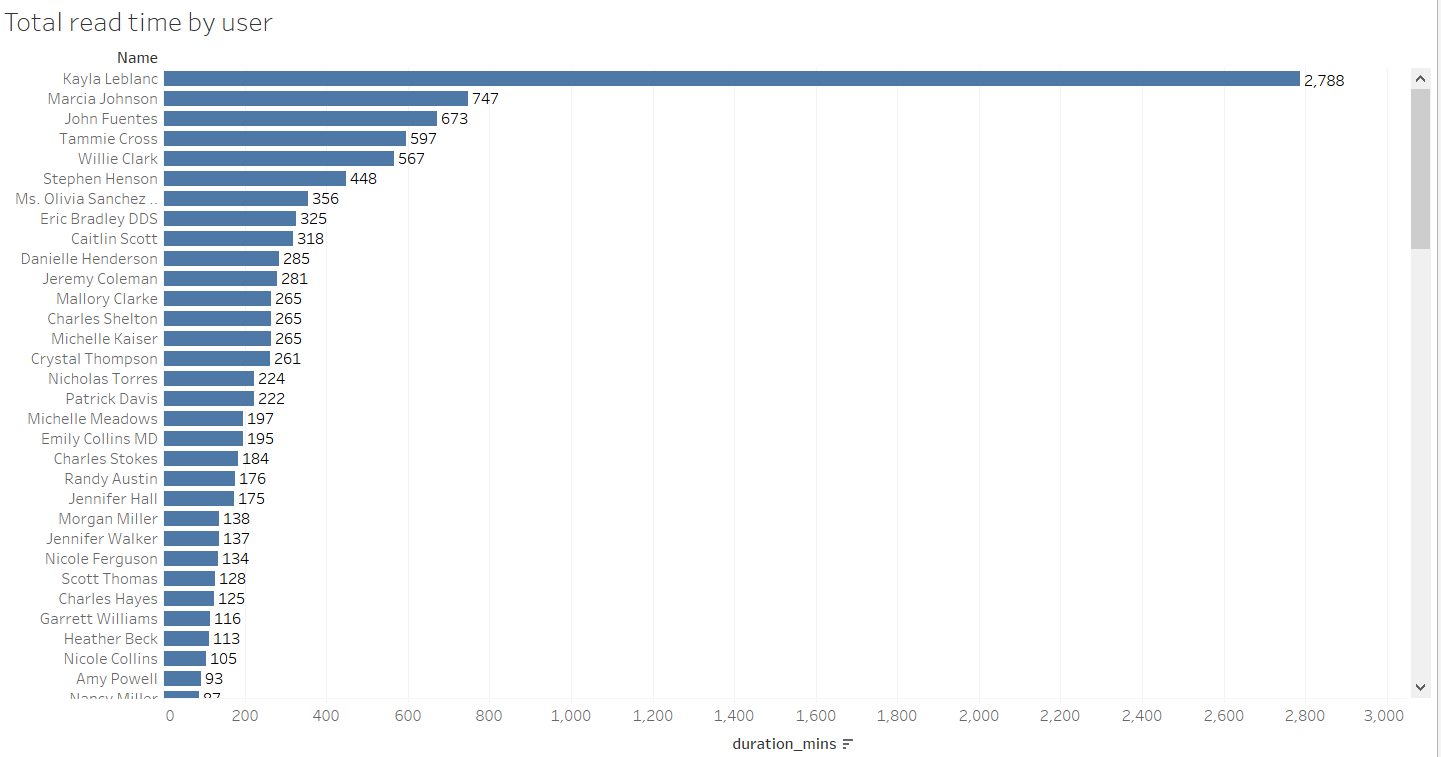
\includegraphics[width=1\linewidth]{gfx/total_read_time_by_user_5min}\label{fig:total_read_time_5min_no_scroll}} \quad 
	\subfloat[Daily activity timeline]
	{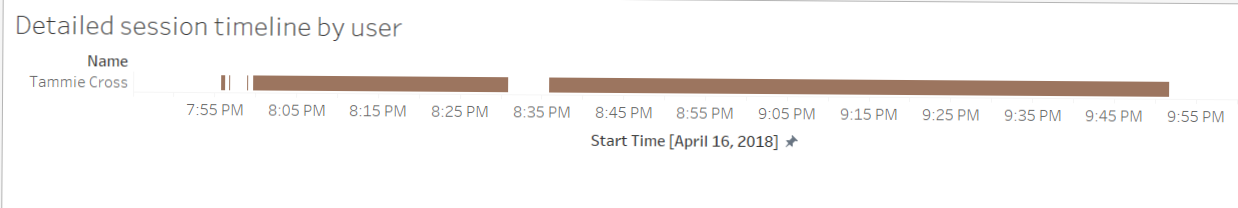
\includegraphics[width=1\linewidth]{gfx/detailed_session_timeline_by_user_5min_no_scroll}\label{fig:detailed_session_timeline_by_user_5min_no_scroll}} \quad
	\caption{Reading session visualizations for session\_timeout of 5 minutes.}\label{fig:visualizations_1st_iteration}
\end{figure}


\subsection{Improving the baseline}
Using the previous settings as a baseline, the next idea was to reduce the value of session\_timeout, because the additional time benefit of 5 minutes might be too much grace time for a user reading without doing any action. Scrolling events are helpful to detect more frequent activity, but they can be overwhelming for the web server and the database, for that reason, the web server callback was limited to maximum 1 call per minute.

Sessions were computed using different parameters for the session\_timeout, and the maximum idle time between user actions inside a session was plotted (figure \ref{fig:idle_time_comparison}).

\begin{figure}[bth]
	\myfloatalign
	\subfloat[1 min]
	{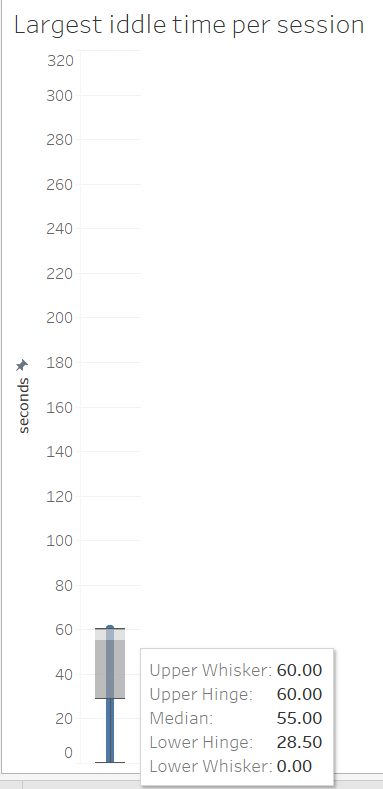
\includegraphics[width=0.19\linewidth]{gfx/largest_iddle_time_1min_timeout}\label{fig:largest_iddle_time_1min_timeout}}  
	\subfloat[2 min]
	{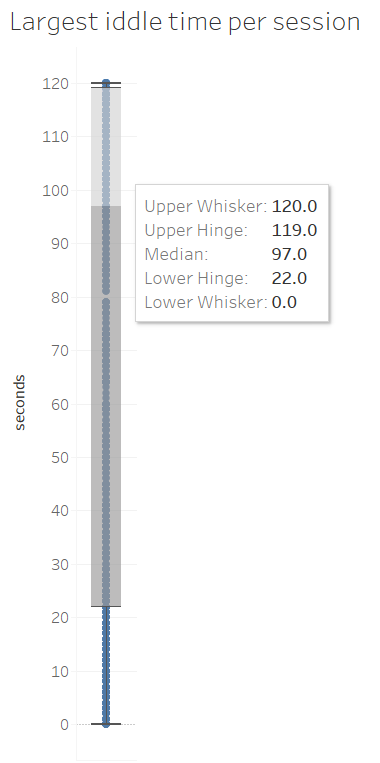
\includegraphics[width=0.19\linewidth]{gfx/largest_iddle_time_2min_timeout}\label{fig:largest_iddle_time_2min_timeout}} 
	\subfloat[3 min]
	{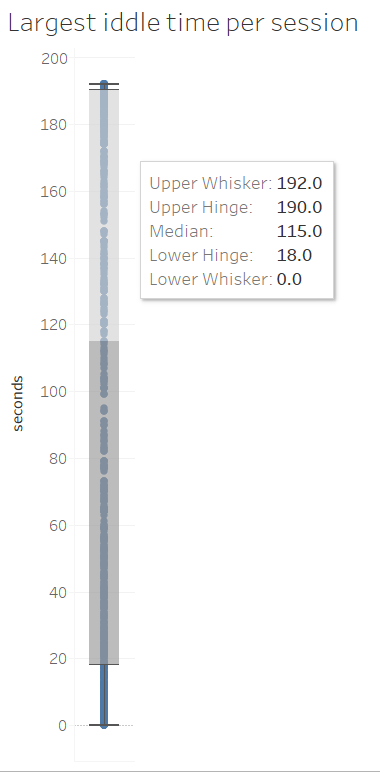
\includegraphics[width=0.19\linewidth]{gfx/largest_iddle_time_3o2min_timeout}\label{fig:largest_iddle_time_3o2min_timeout}}
	\subfloat[4 min]
	{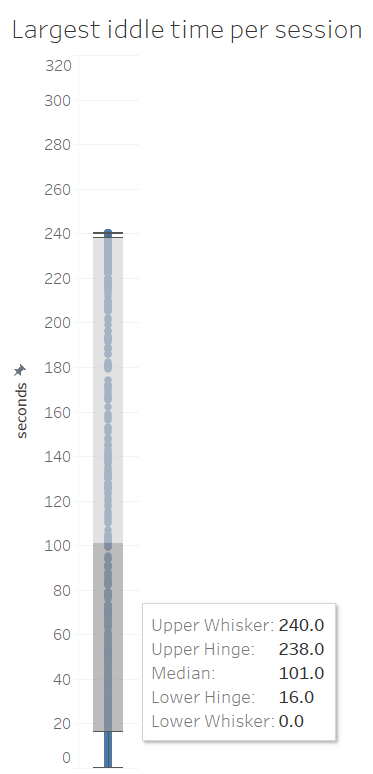
\includegraphics[width=0.19\linewidth]{gfx/largest_iddle_time_4min_timeout}\label{fig:largest_iddle_time_4min_timeout}} 
	\subfloat[5 min]
	{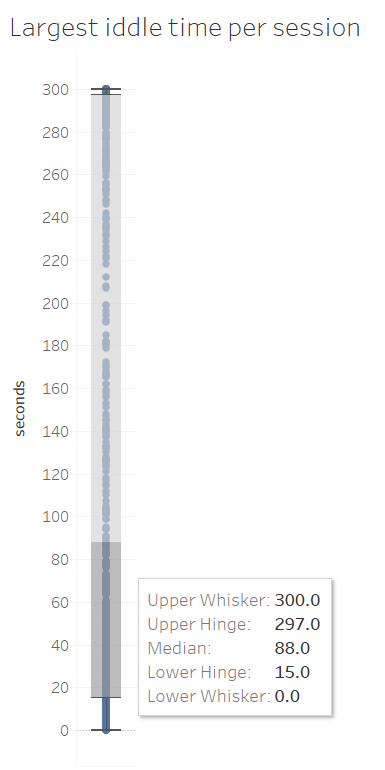
\includegraphics[width=0.19\linewidth]{gfx/largest_iddle_time_5min_timeout_v2}\label{fig:largest_iddle_time_5min_timeout_v2}} \quad
	
	\caption{Box plot of maximum idle time per session, for distinct session timeout values}\label{fig:idle_time_comparison}
\end{figure}

We can observe that the median value fluctuates between 90 and 120 seconds (as shown in table \ref{tb:table_median_value}). By taking this value into account and some empirical measures, the value of the timeout was set to 2 minutes. 

The upper hinge, however, increases as the timeout value do. This is because small sessions are stitched together, therefore moving the value upwards.

\begin{table}[htb]
	\begin{tabularx}
		{\textwidth}{Xllll}\toprule
		\tableheadline{Timeout value (min)} & 
		\tableheadline{Median (sec)} &
		\tableheadline{Upper hinge(sec)} \\ 
		\midrule 
		1 & 55 & 60 \\ 
		\hline 
		2 & 97 & 119 \\ 
		\hline
		3.2 & 115 & 190\\ 
		\hline 
		4 & 101 & 238\\ 
		\hline 
		5 & 88 & 297\\ 
		\hline 
	\end{tabularx} 
	\caption{Maximum idle time statistics with different session timeout values}\label{tb:table_median_value}
\end{table}

By comparing the total time per user between the baseline and the final settings (figure \ref{fig:total_time_comparison}), we can observe that a reduction of almost 300\% in the total time per user was achieved. This means that the previous session\_timeout value was too big, therefore computing times longer than what they really were.

\begin{figure}[!htb]
	\myfloatalign
	\subfloat[Baseline (5 minutes)]
	{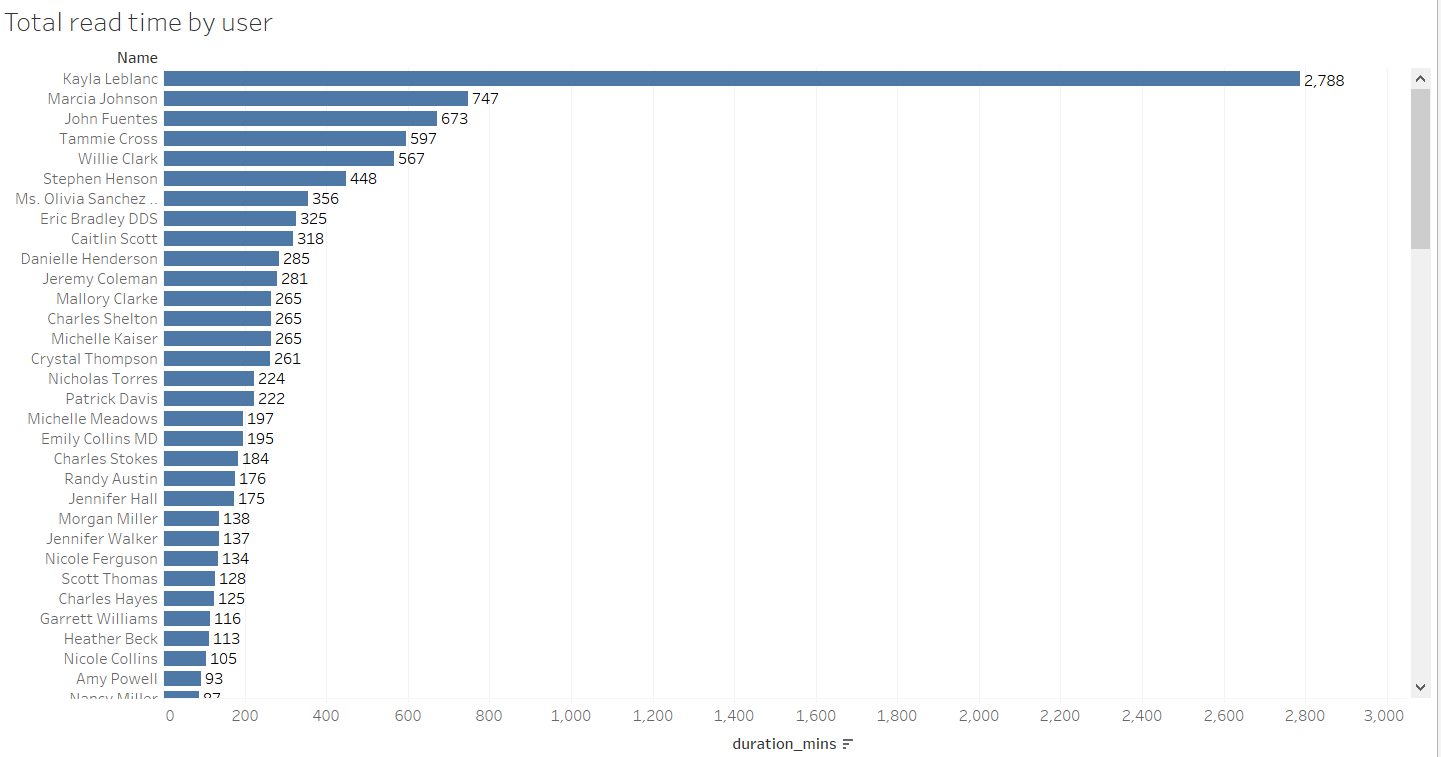
\includegraphics[width=1\linewidth]{gfx/total_read_time_by_user_5min}\label{fig:total_read_time_by_user_5min}} \quad 
	\subfloat[Final settings (2 minutes)]
	{
	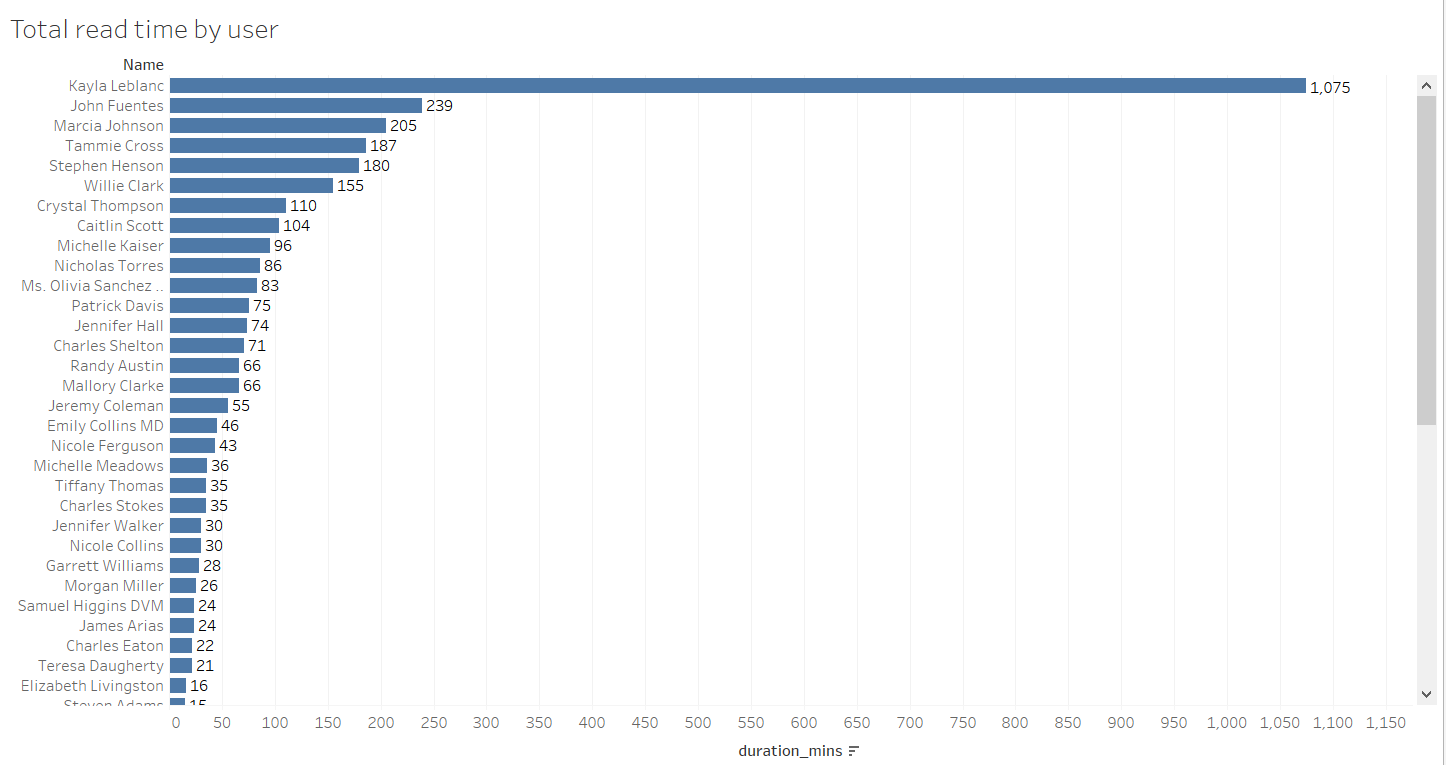
\includegraphics[width=1\linewidth]{gfx/total_read_time_by_user_2min}\label{fig:total_read_time_by_user_2min}} \\
	\caption{Total time improvement comparison}\label{fig:total_time_comparison}
\end{figure}

Finally, for the detailed activity, a big change is observed, in figure \ref{fig:detailed_session_5min}, we observe roughly two smooth reading sessions, which later, with a finer session detection gets split into smaller reading sessions (figure \ref{fig:detailed_session_2min}). This means that we correctly detected the user's gap of attentions, therefore a more precise session time was measured.

\begin{figure}[!htb]
	\myfloatalign
	\subfloat[Baseline (5 minutes)]
	{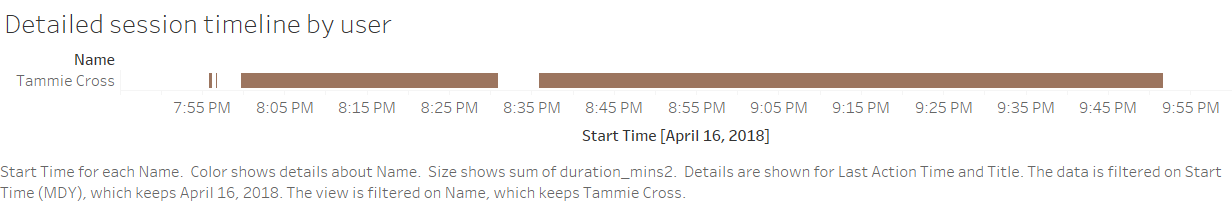
\includegraphics[width=1\linewidth]{gfx/detailed_session_timeline_by_user_5min}\label{fig:detailed_session_5min}} \quad 
		
	\subfloat[Final settings (2 minutes)]
	{
	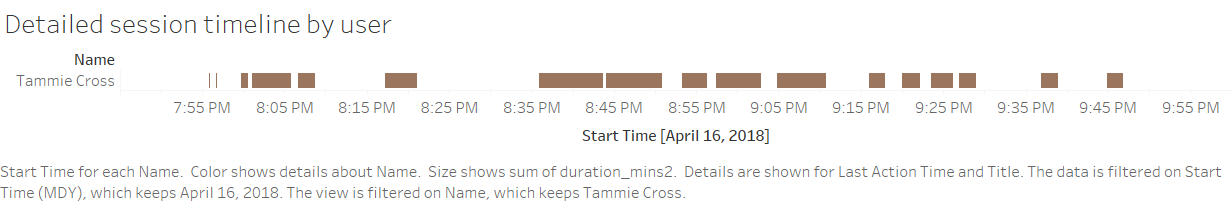
\includegraphics[width=1\linewidth]{gfx/detailed_session_timeline_by_user_2min}\label{fig:detailed_session_2min}} \\
	\caption{Low level session tracking time line}\label{fig:detailed_session_comparison}
\end{figure}


\subsection{Validation}
Before the implementation of the session tracking, students manually reported the time spent reading in Zeeguu. Therefore a useful validation of the computed session tracking is against the reported time by students.
In table \ref{tb:comparison_read_time} we can observe the difference between those times. There is a clear difference in the obtained results.

\begin{table}[!htb]
	\begin{tabularx}
		{\textwidth}{Xllll}\toprule
		\tableheadline{Student} & 
		\tableheadline{Reported time} &
		\tableheadline{Computed time} \\ 
		\midrule 
		Student 1
		 & 11 hours
		  & 59 minutes
		   \\ 
		\hline 
		Student 2
		 & 1.5 hours
		  & 44 minutes
		   \\ 
		\hline
		Student 3
		 & 4 hours
		  & 54 minutes
		  \\ 
		\hline 
	\end{tabularx} 
	\caption{Comparison of reading time reported by students vs the time computed by the algorithm (using a timeout value of 2 minutes)}\label{tb:comparison_read_time}
\end{table}

\section{Exercise session experiments}
For the exercise sessions, the implementation is quite simple. Only two events are tracked:
\begin{itemize}
	\item Answering the exercise (either right or wrong)
	\item Asking for a hint
\end{itemize}

The only parameter to define is the exercise session\_timeout. For the exercises, we know that they are short and quick activities, which take only a couple of second to provide an answer. Therefore the timeout must be much smaller than for reading.

In this case, the time between the exercise opening and the answering is computed by a timer. Therefore by a descriptive analysis of the answering time (box plot in figure \ref{fig:exercise_solving_speed}). The obtained results are 6, 10 and 21 seconds, which represent the median, upper hinge and upper whisker. These metrics represent the 50\%, 75\% and 100\% of a normally distributed population. 

\begin{figure}[bth]
	\centering
	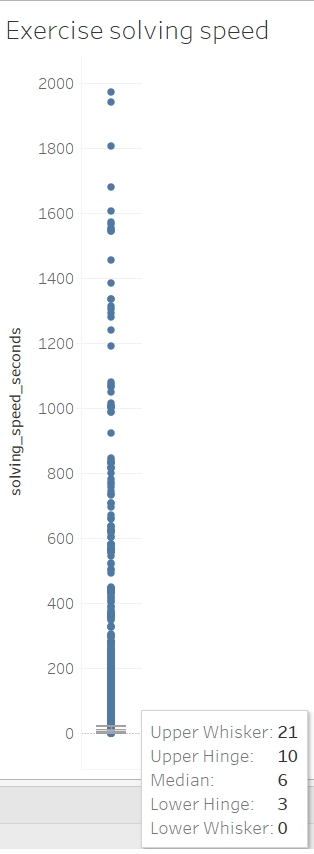
\includegraphics[width=0.2\linewidth]{gfx/exercise_solving_speed}
	\caption{Exercise time box plot}\label{fig:exercise_solving_speed}
\end{figure}

Given that the tracked time window is so small, a final setup of no grace time but using the upper whisker value (21 seconds) is chosen.




%************************************************
\chapter{Discussion}
%************************************************
After the implementation of session tracking, useful information about time and quality of work can be presented to teachers and students. Example of questions and analysis that can now be performed with the session tracking are presented in this chapter.
With this knowledge they can adjust their teaching strategy and have a better understanding of how the class is using the system.

\section{Reading session}

By visualizing the amount of time spent for the students in a class, we can detect "islands" of activity common for the whole class (Figure \ref{fig:class_heatmap_by_date}). These can be explained with a visualization by week day. In Figure \ref{fig:class_heatmap_by_weekday} we can confirm that the students are mostly actively reading on Sundays and Mondays.

\begin{figure}[bth]
	\myfloatalign
	\subfloat[Heat map of time spent by day and user in a class]
	{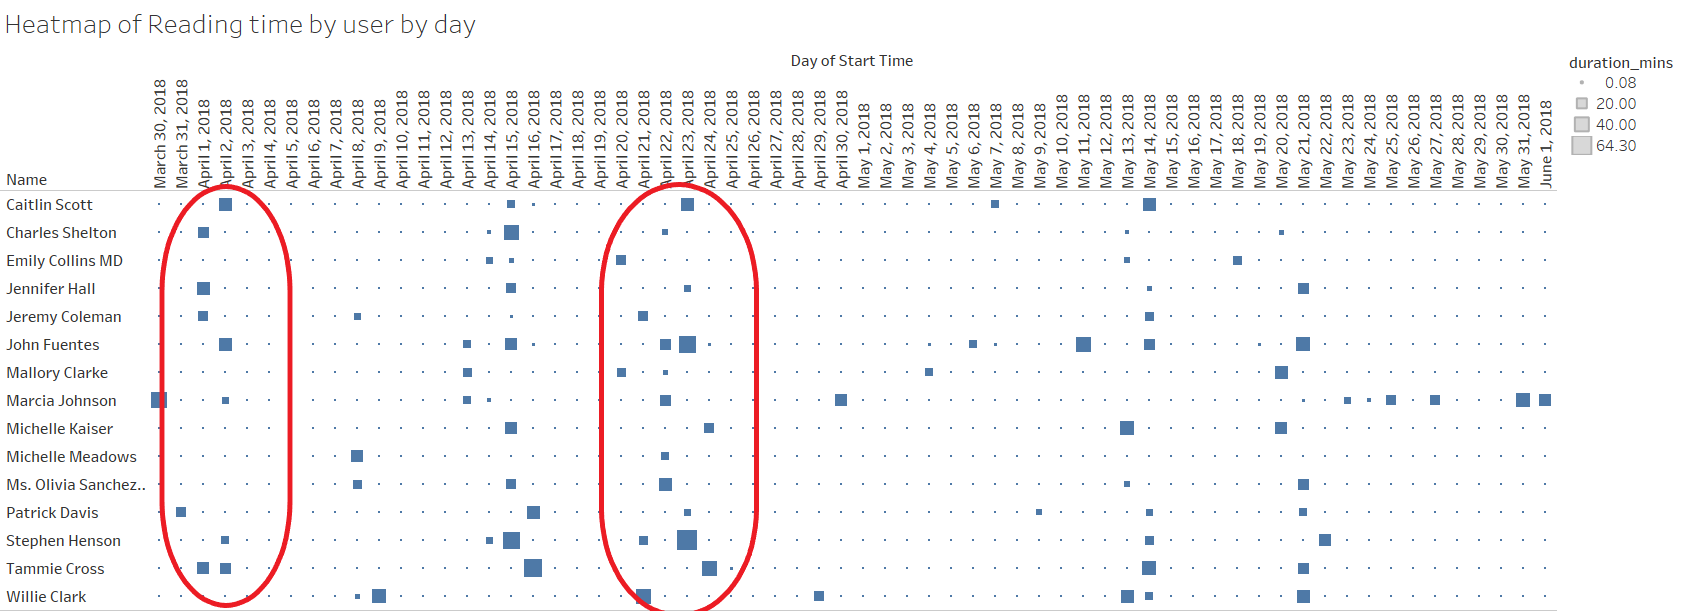
\includegraphics[width=.45\linewidth]{gfx/Heatmap_by_user}\label{fig:class_heatmap_by_date}} \quad 
	\subfloat[Heat map of time spent by weekday and user in a class]
	{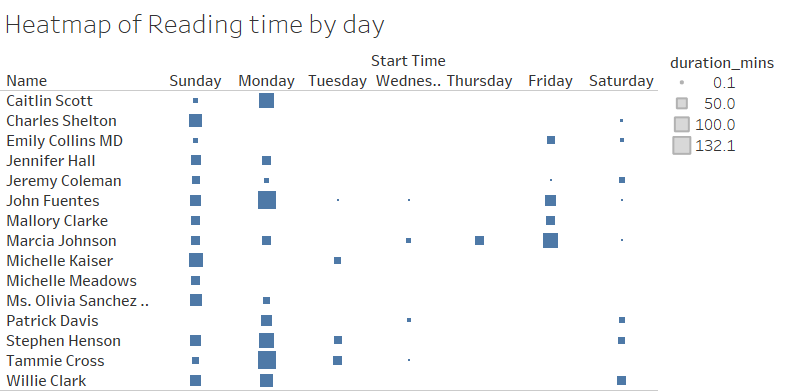
\includegraphics[width=.45\linewidth]{gfx/Reading_time_by_weekday}\label{fig:class_heatmap_by_weekday}} \quad
	\caption{Total time spent by a class, analyzed by date}
\end{figure}


Since the reading sessions are associated to an article, an analysis of the time spent by article can be performed. In Figure \ref{fig:treemap_by_article} we display the total amount of time spent by a class of students learning Dutch. With this information the teacher can observe which articles are the ones that most students have read, and also from which source they read, so a further discussion in class about the content can be done.

\begin{figure}[h]
	\centering
	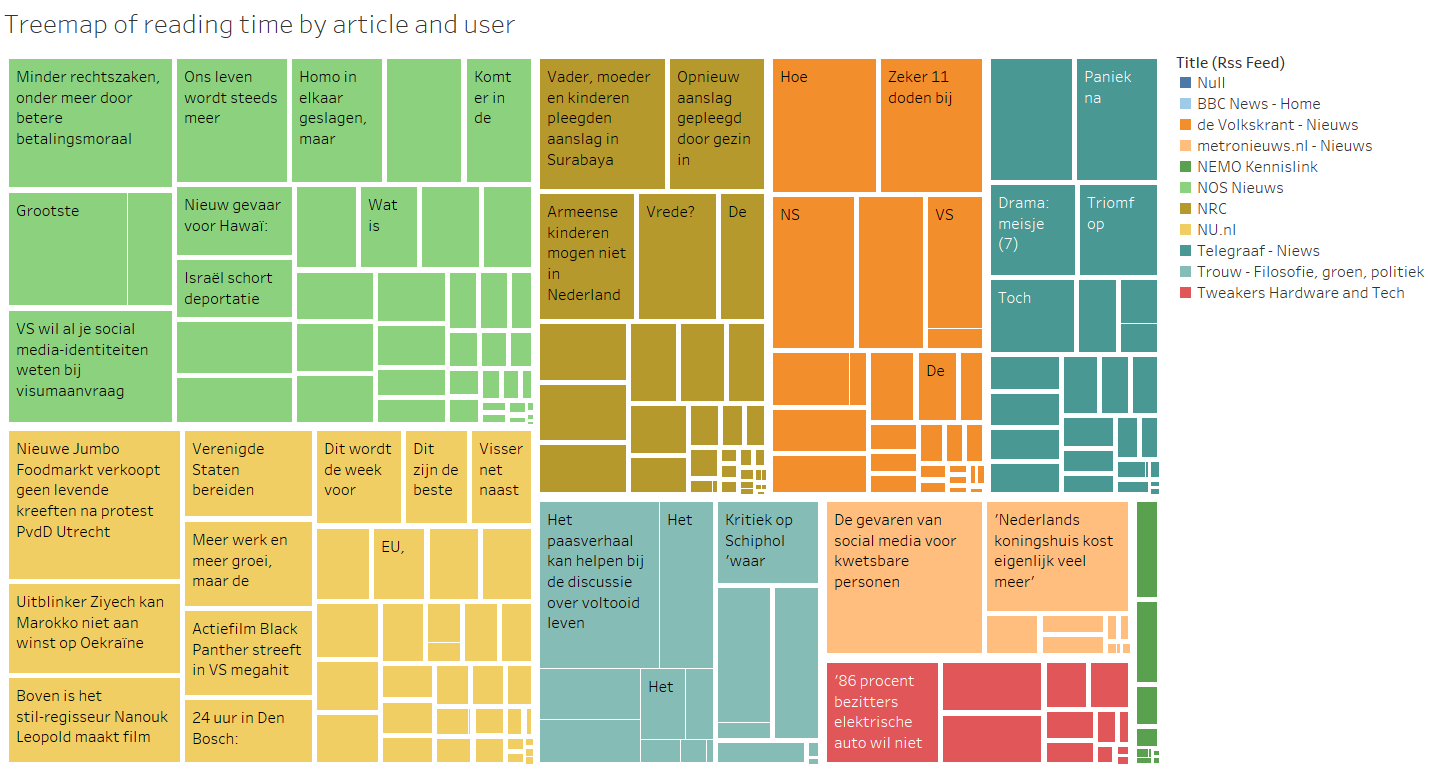
\includegraphics[width=1\linewidth]{gfx/Treemap_by_article}
	\caption{Treemap of time spent by article. The color indicates the source of the article. Each block represents a user and the size represents the total time spent by a user on that article}
	\label{fig:treemap_by_article}
\end{figure}

%An alternative way of grasping an idea about text difficulty and quality of work can be done based on the time students spend on average reading an article. In Figure \ref{fig:boxplot_by_article}, we can observe that most of the articles were read during less than ten minutes, amongst which the majority are concentrated in less than 4 minutes sessions.
%
%\begin{figure}[h]
%	\centering
%	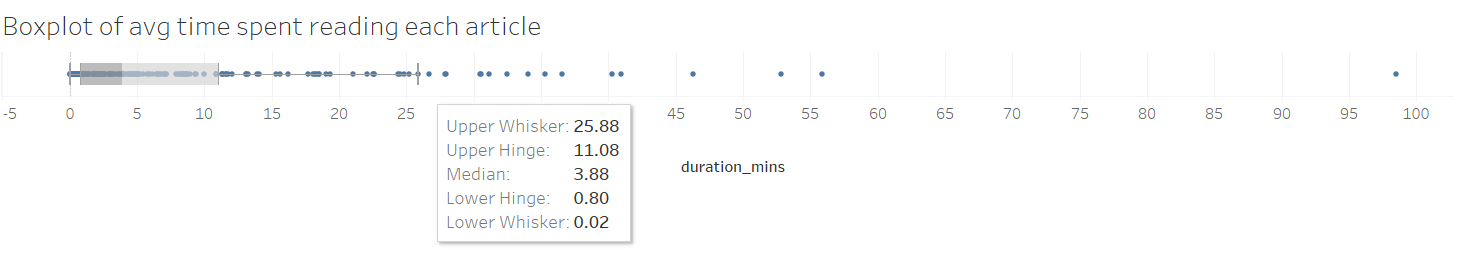
\includegraphics[width=0.7\linewidth]{gfx/avg_time_spent_by_article}
%	\caption{Box plot of the average time required to read an article. It shows that most articles are read in less than 10 minutes and that there are some articles that take more time}
%	\label{fig:boxplot_by_article}
%\end{figure}

And at the individual level, the user can visualize and understand his own work, in order to be aware of his own progress. In Figure \ref{fig:Personal_dashboard}, an example of a dashboard containing the information that could be relevant for a user is displayed.

\begin{figure}[!htb]
	\centering
	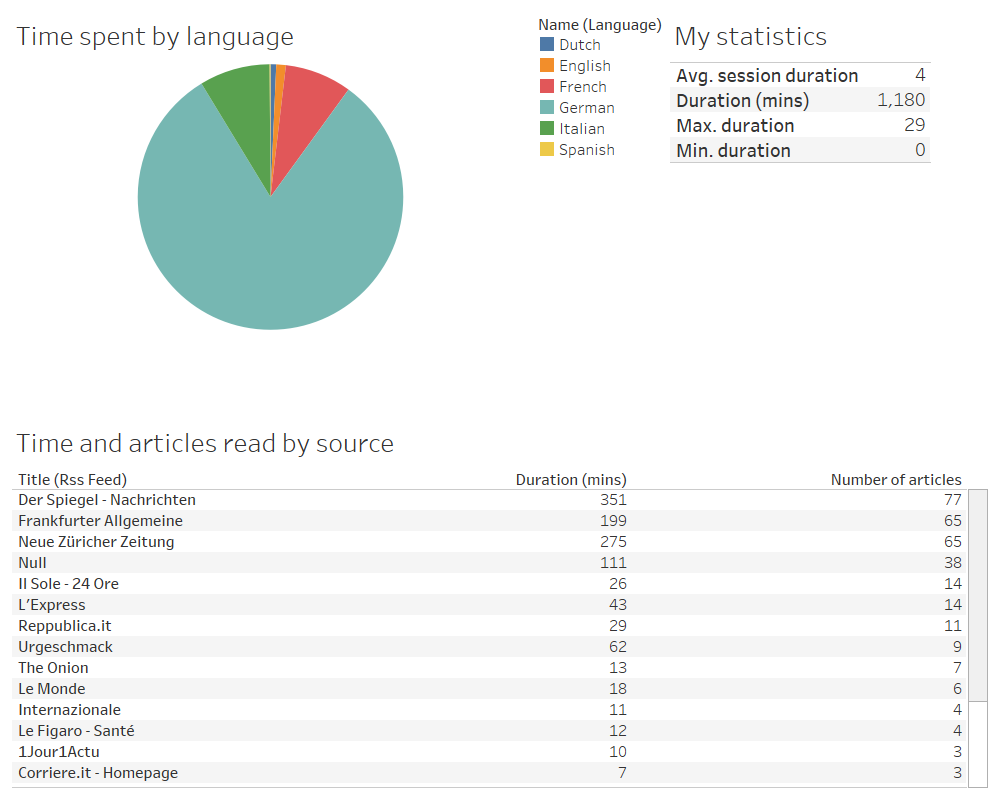
\includegraphics[width=1\linewidth]{gfx/Personal_dashboard}
	\caption{Dashboard displaying individual statistics about reading habbits}
	\label{fig:Personal_dashboard}
\end{figure}



\section{Exercise session}
Typical questions related to the exercises are how much time has the student being practicing? Do they practice daily? For how long? Etc. In this chapter a list of analysis based on time spent on exercises is shown and discussed.

The first question is how much time the class is spending on practicing their vocabulary? With a simple bar chart we can visualize and compare how much time in total has the class spent practicing, and also who has been putting more effort on it. As we can observe in Figure \ref{fig:Total_exercise_time}, some students really like to rehearse their new vocabulary, while the rest have lost their interest over time.

\begin{figure}[bth]
	\centering
	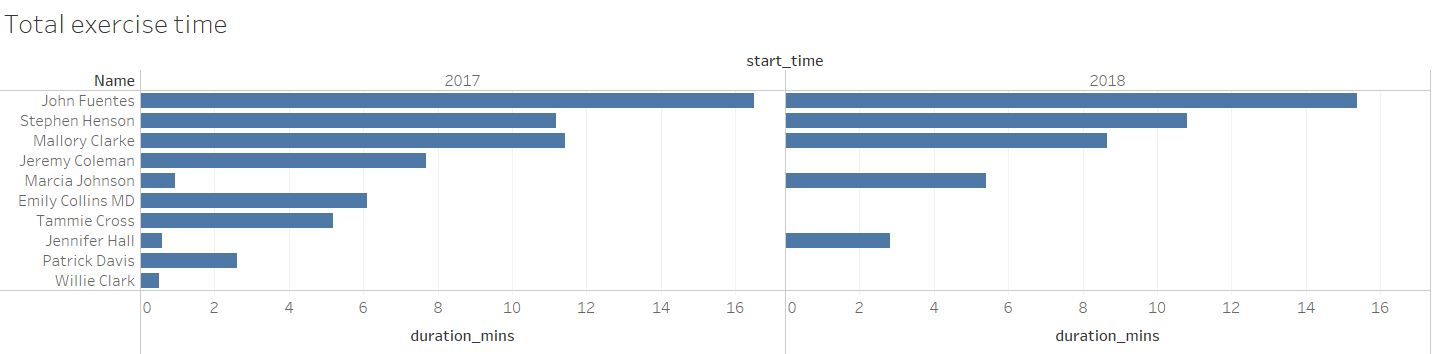
\includegraphics[width=1\linewidth]{gfx/Total_exercise_time}
	\caption{Class exercise time year over year comparison}
	\label{fig:Total_exercise_time}
\end{figure}

If the interest is on when do the students practice, a visualization by weekday can show us that, for example, for a particular class, most of the students prefer to practice on Wednesday (Figure \ref{fig:Class_exercise_by_weekday}).

\begin{figure}[bth]
	\centering
	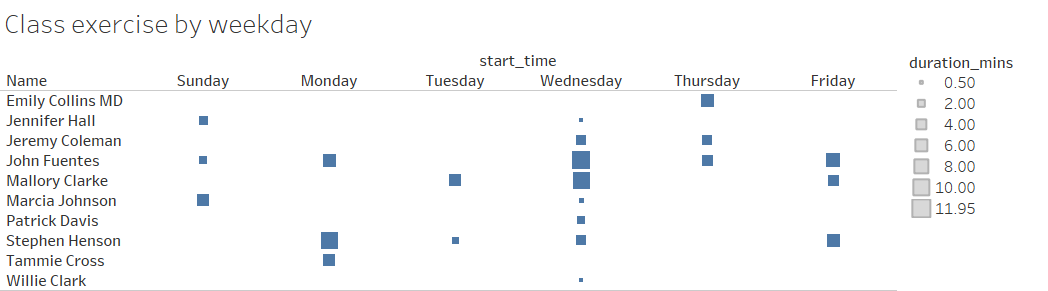
\includegraphics[width=1\linewidth]{gfx/Class_exercise_by_weekday}
	\caption{Class exercise heatmap by weekday}
	\label{fig:Class_exercise_by_weekday}
\end{figure}

For understanding the quality of the practice, we can also visualize the average session length. An interesting finding, as we can see in Figure \ref{fig:Avg_exercise_session_duration}, is that on average the exercise sessions are 2.2 minutes long. Some of the students however practice for less than a minute, this can tell us about their commitment with the activity or about their knowledge, since exercises have fixed number of questions, and thus, a fast student will finish faster. By observing these results a teacher can encourage the class to practice for at least a certain amount of minutes in a row, in order to keep a better focus. Finally, this visualization can also be used to avoid students gaming the system by opening the application multiple times but not really focusing on the assignment.
The finding about the average session time is also a good indicator about how the exercise session\_timeout should be configured.

\begin{figure}[bth]
	\centering
	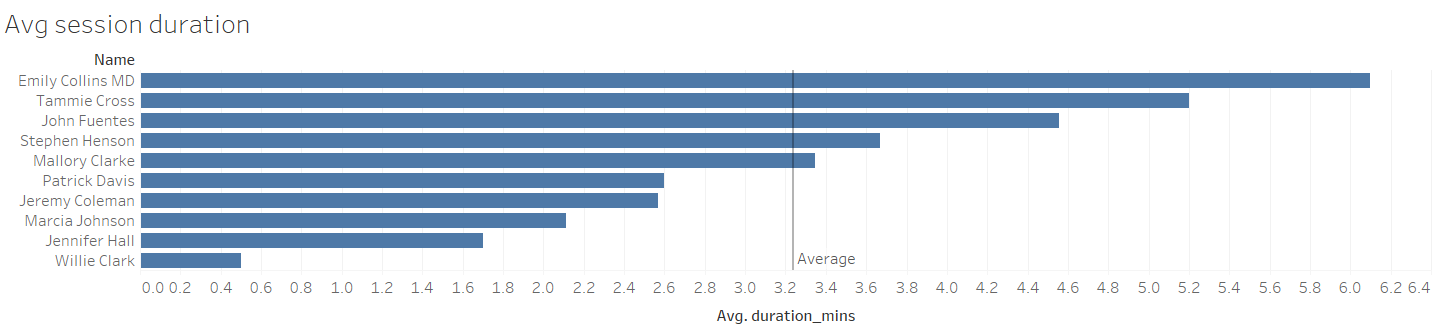
\includegraphics[width=1\linewidth]{gfx/Avg_exercise_session_duration}
	\caption{Class average session duration}
	\label{fig:Avg_exercise_session_duration}
\end{figure}

Continuing with the analysis of the working habits, a detailed time line (Figure \ref{fig:Exercise_timeline}) is a more fine grained visualization, where a teacher can observe at what time of the day the students practiced and if they worked uninterruptedly or not.

\begin{figure}[!h]
	\centering
	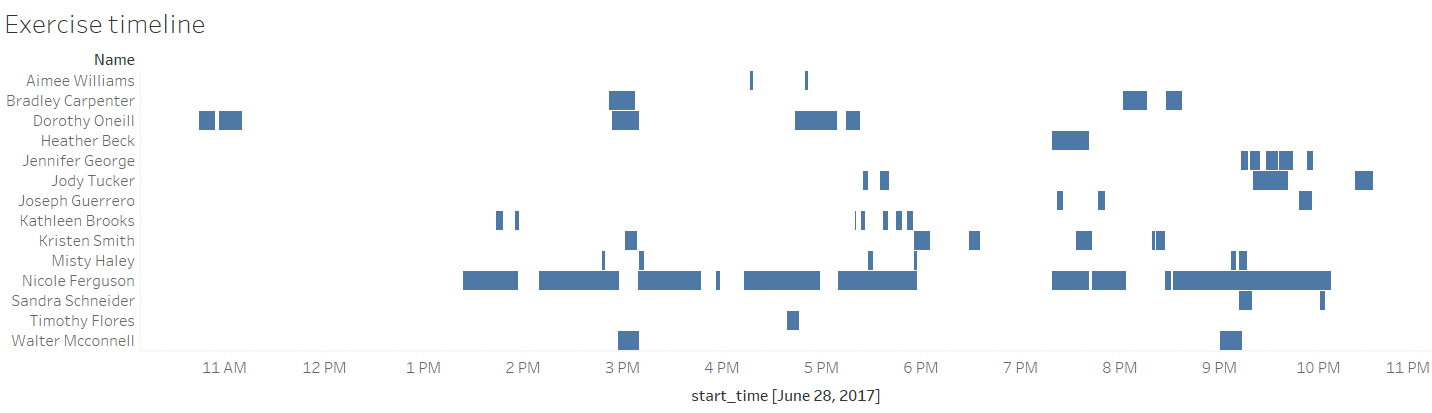
\includegraphics[width=1\linewidth]{gfx/Exercise_timeline}
	\caption{Class exercise time line}
	\label{fig:Exercise_timeline}
\end{figure}

As well, from the individual perspective, a student can observe how is his progress and consistency over time. He can set himself personal goals and track over time how is his performance. In Figure \ref{fig:Session_durations_by_user} we observe that the student was not constant in his daily practice.

\begin{figure}[!h]
	\centering
	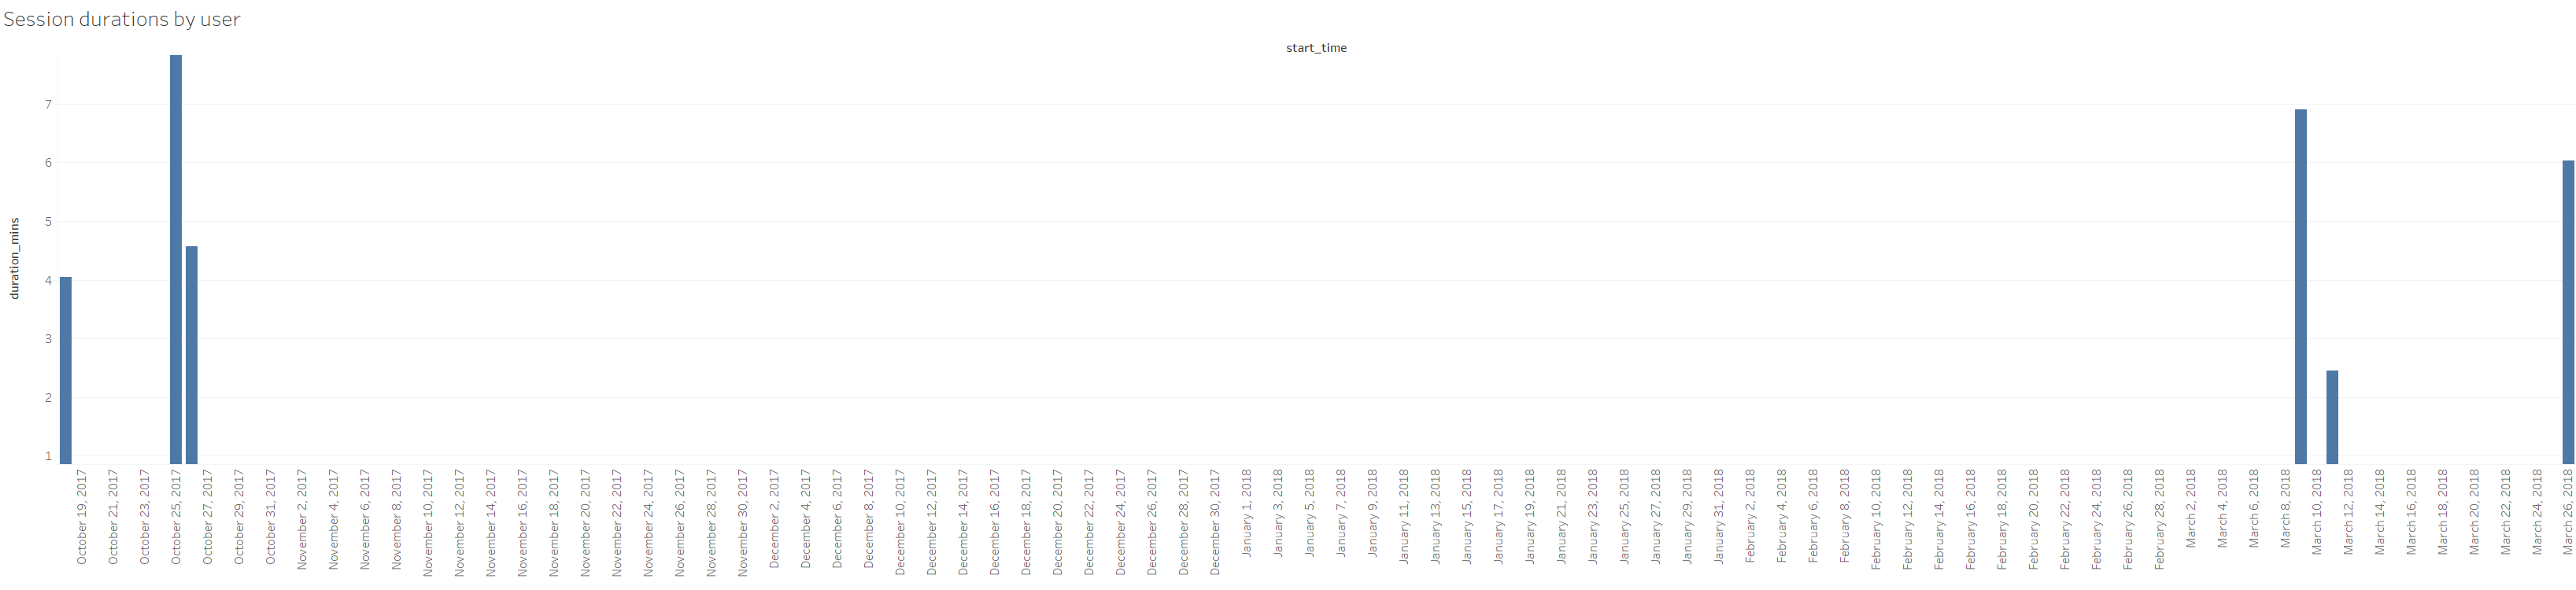
\includegraphics[width=1\linewidth]{gfx/Session_durations_by_user}
	\caption{Heat map showing exercise time calendar}
	\label{fig:Session_durations_by_user}
\end{figure}

%************************************************
\chapter{Conclusion}
%************************************************

As observed in section \ref{p03:results}, not only the time spent but also the quality of the work can be assessed with a precise session tracking. A teacher can use multiple approaches to evaluate the progress of students in the individual level and also as a class.

The extensibility and applicability of the session tracking algorithm is vast. The proposed algorithm can be used for other purpose ITS, by only adjusting the timeout and the particular set of rules for the specific application. As well as for the commercial industry, the session tracking algorithm can be used to track customers engagement with a particular website, and interesting questions can be crafted and answered via visualizations. In the office, session tracking can also be implemented to detect employees who are having too much distraction from their activities. 

For our particular application, the Zeeguu platform, one of the main goals was to keep students from gaming the system. With that goal in mind the event tracking and the timeout parameters had to be strict. However, not for every application must be the same.

Finding the optimal timeout value is not a trivial task, it requires sample data and multiple tests to find a good setting, and even then, it can vary from context to context (\Eg depending on the level of expertise of users, on the type of ITS, on the level of trust that can be placed on users, etc).


%************************************************
\chapter{Future Work}
%************************************************


Reading speed (also for filtering reading articles estimated reading time)

Move to prescriptive analytics


%%\include{multiToC} % <--- just debug stuff, ignore for your documents
% ********************************************************************
% Backmatter
%*******************************************************
\appendix
%\renewcommand{\thechapter}{\alph{chapter}}
%\cleardoublepage
%\part{Appendix}\label{pt:appendix}
\chapter{Appendix}\label{pt:appendix}
%************************************************
\section*{Interview A}\label{interview01}
%************************************************
\begin{itemize}

	\item \textit{Question: What kind of information would you like to get and what is the purpose?}

I give a lot of freedom to my students to choose their activities. I don't mind what they do as long as they are reading. That is a very modern approach to language teaching so they are exposed a lot to the language, and the only thing I want is that they spend for example half an hour a day or an hour a week on reading, and I award them with points for every half hour of work. They have to get 60 points a year for example.
They get to choose for reading activities, speaking activities or writing activities. When it comes to reading activities that is when Zeeguu comes in. A number of students are very fond of Zeeguu, they don't do anything else for reading, so they spend a couple of hours or minutes on the system reading, checking for translations, doing exercises. My students are very motivated but even motivated students, when the deadline approaches tend to become less motivated to do the things right away. They tend to become a bit more easy on the honesty, so when the deadline approaches they might be doing something during 10 minutes and they report on the paper that they spent 60 minutes. I say to my students I cannot look into your head, I cannot see what's happening in your head, I cannot see what you're doing in terms of language acquisition the only thing I can see is that you spent an amount of time on reading activities. That is where this dashboard might be a little more helpful than now, because now I only have their words, so they fill out the report saying for example that they spend 30 minutes or 60 minutes on a certain text I can look into the system and I can see the difficulty of the text and I can see how many words they have asked for a translation but that's all. So what I need is more things that give me the idea that they really worked for example 30 minutes. I need to be convinced that they are doing that amount of time. 
I don't see anything on their activities like their exercises, the time if that is possible. 
I don't think it's fair when I don't convince my students that I have serious instruments that can make a positive guess about their work. When I don't do that I leave it to their self-discipline and I don't think it's fair to the students. They need to have some kind of guidance, so I have to put a little pressure on them to do the right thing.

	\item \textit{Question: So that reinforces the idea that both you and your students can see the same information and they can realize that this is what the professor is going to visualize, so maybe I have to put a little extra effort?}
	
Yeah that would be very nice.

	\item \textit{Question: Talking about the weekly report that you mentioned, you only ask them how many hours they worked? }

They fill out of this form telling me their name, the classroom, the date that they did this activity, the text title, the magazine they chose the text from and how many minutes, 30 or 60 minutes.

	\item \textit{Question: I'm just trying to understand the purpose behind the report, one side is for keep track of what they are doing but is it also for motivating?}
	
Yes it's external motivation, because most of students don't like to do homework when they are home they want to do other things. I have to put pressure on them to do the things they really should do in order to get to the exam. so I have chosen for a system in which I can rely on them to do things at home by giving them 60 points for 30 hours, that means about one hour a week, and as a personalized system they can choose whatever activity they want to do. In the end, when they don't have the 60 points they can't go to the next year.

	\item \textit{Question: The next question is how will you measure the quality of their work? Would it be only the amount of time do they spend reading? Or as well the score on the exercises? Or do you have another way of evaluating the quality?}
	
Now I only have quantitative measures I can look at the text, I can look at what words they have been asking to be translated and that gives me an idea about the quality of their work. Sometimes I see that they ask for too easy words and I talk to them about it. Whenever I see something that I don't like I write down the names and after class I ask them to come, and I ask them "why did you look up that word? You know this word, or at least I think you should know this word". From time to time, I have a discussion with those students to probe quality, but that is difficult because when I say "I think you have learnt these words in the first class 4 years ago", they can say "well, I forgot" and there is nothing I can do about it. I keep asking those questions and when I ask those questions that is a way I put pressure, they know that if they take it too easy I can ask a lot of questions that they don't like so they are triggered to do their best I think.
But it might be helpful indeed to have some information about how they performed in those exercises.

	\item \textit{Question: And after how many correct exercises of a specific word would you say that they have learned the word? We can ask them ten times the same word and maybe after the fifth time they have learned the world already.}
	
That is a very difficult question; the basis of the approach that I use is statistical learning. They see words, they see texts, they see language, and they make inductions about that, and every time whenever they see it for the second, third, fourth time it is enhanced, that meaning is best kept in mind, so every repetition is welcome.
It's a bit compared to when you learn your mother tongue you have a lot of exposure to the language, the amount of exposure is so enormous to the first language and I don't get that the amount of exposure with my students because I only have three classes a week.

	\item \textit{Question:Are you interested in analyzing individual students, or as a class or both?}
	
Individual in the first place because it's personalized, but to have information about how a class performs might be helpful as well.
I have for example two classes one of them is very loyal, always have the points on time and the other group doesn't. That is something that I see and this will be reinforced by information; but for me it's not necessary because I evaluate them on the individual level. 
And the second problem is that not every student uses Zeeguu to get his points.

	\item \textit{Question:Another question will be what level of detail are you interested? For example at the word level or a bit more general for example at the session level, and how many sessions or how much time have they spent? }
	
The amount of time they spend on the system is very important, I think. 
And the amount of hours they do during the exercises might be a good indicator of their effort. When they are having a lot of errors, they are not having a mental activity they are just choosing whatever. When they are busy reading they are busy with meaning. 

	\item \textit{Question:How often did you evaluate their work? Is it a daily, weekly, monthly?}
	
Two monthly. I have five times a year so I have 5 deadlines and that is in terms of 2 months. I asked for example 12 points by the end of the first two months. And if they don't, they get an application with me to do two points a week. I work with levels: orange, green and red so when you are on level green you're ok, you can choose whatever you want, and when you don't meet my demands you go to level orange. That means every week you have to produce two points. And after the second time that they don't reach the deadline, they go to level red.

	\item \textit{Question: This question is related to analyzing the students as a class. Are you interested in detecting special students like the ones that are working a lot?}
	
It doesn't tell me much because some students don't use the system. What might be interesting is that the students might be able to see the ranking of the articles. The ones that they like a lot. Maybe that can be done in the system. It saves a lot of time to them because I have to look at the text and decide which one to take. And with a lot of extra information from other students, it might save time. 

	\item \textit{Question:Is there something that you would like to add?}
	
Normally teachers give homework that is not personalized. Students have text in the book for example or text from the internet that is copied and they work with that. What might be a good addition for these colleges for example is that the teacher chooses a text and designs a sort of test to be able to verify that they have done the work and that is of quality. I am not really interested in quality but in quantity.
\end{itemize}
%************************************************
\chapter{Interview B}
%************************************************
%********************************************************************
% Other Stuff in the Back
%*******************************************************
%********************************************************************
% Bibliography
%*******************************************************
% work-around to have small caps also here in the headline
% https://tex.stackexchange.com/questions/188126/wrong-header-in-bibliography-classicthesis
% Thanks to Enrico Gregorio
\defbibheading{bibintoc}[\bibname]{%
  \phantomsection
  \manualmark
  \markboth{\spacedlowsmallcaps{#1}}{\spacedlowsmallcaps{#1}}%
  \addtocontents{toc}{\protect\vspace{\beforebibskip}}%
  \addcontentsline{toc}{chapter}{\tocEntry{#1}}%
  \chapter*{#1}%
}
\printbibliography[heading=bibintoc]

% Old version, will be removed later
% work-around to have small caps also here in the headline
%\manualmark
%\markboth{\spacedlowsmallcaps{\bibname}}{\spacedlowsmallcaps{\bibname}} % work-around to have small caps also
%\phantomsection
%\refstepcounter{dummy}
%\addtocontents{toc}{\protect\vspace{\beforebibskip}} % to have the bib a bit from the rest in the toc
%\addcontentsline{toc}{chapter}{\tocEntry{\bibname}}
%\label{app:bibliography}
%\printbibliography

%%*******************************************************
% Declaration
%*******************************************************
\refstepcounter{dummy}
\pdfbookmark[0]{Declaration}{declaration}
\chapter*{Declaration}
\thispagestyle{empty}
Put your declaration here.
\bigskip

\noindent\textit{\myLocation, \myTime}

\smallskip

\begin{flushright}
    \begin{tabular}{m{5cm}}
        \\ \hline
        \centering\myName \\
    \end{tabular}
\end{flushright}

%\cleardoublepage\pagestyle{empty}

\hfill

\vfill


\pdfbookmark[0]{Colophon}{colophon}
\section*{Colophon}
This document was typeset using the typographical look-and-feel \texttt{classicthesis} developed by Andr\'e Miede and Ivo Pletikosić.
The style was inspired by Robert Bringhurst's seminal book on typography ``\emph{The Elements of Typographic Style}''.
\texttt{classicthesis} is available for both \LaTeX\ and \mLyX:
\begin{center}
\url{https://bitbucket.org/amiede/classicthesis/}
\end{center}
Happy users of \texttt{classicthesis} usually send a real postcard to the author, a collection of postcards received so far is featured here:
\begin{center}
\url{http://postcards.miede.de/}
\end{center}
Thank you very much for your feedback and contribution.

\bigskip

\noindent\finalVersionString

%Hermann Zapf's \emph{Palatino} and \emph{Euler} type faces (Type~1 PostScript fonts \emph{URW
%Palladio L} and \emph{FPL}) are used. The ``typewriter'' text is typeset in \emph{Bera Mono},
%originally developed by Bitstream, Inc. as ``Bitstream Vera''. (Type~1 PostScript fonts were made
%available by Malte Rosenau and
%Ulrich Dirr.)

%\paragraph{note:} The custom size of the textblock was calculated
%using the directions given by Mr. Bringhurst (pages 26--29 and
%175/176). 10~pt Palatino needs  133.21~pt for the string
%``abcdefghijklmnopqrstuvwxyz''. This yields a good line length between
%24--26~pc (288--312~pt). Using a ``\emph{double square textblock}''
%with a 1:2 ratio this results in a textblock of 312:624~pt (which
%includes the headline in this design). A good alternative would be the
%``\emph{golden section textblock}'' with a ratio of 1:1.62, here
%312:505.44~pt. For comparison, \texttt{DIV9} of the \texttt{typearea}
%package results in a line length of 389~pt (32.4~pc), which is by far
%too long. However, this information will only be of interest for
%hardcore pseudo-typographers like me.%
%
%To make your own calculations, use the following commands and look up
%the corresponding lengths in the book:
%\begin{verbatim}
%    \settowidth{\abcd}{abcdefghijklmnopqrstuvwxyz}
%    \the\abcd\ % prints the value of the length
%\end{verbatim}
%Please see the file \texttt{classicthesis.sty} for some precalculated
%values for Palatino and Minion.
%
%    \settowidth{\abcd}{abcdefghijklmnopqrstuvwxyz}
%    \the\abcd\ % prints the value of the length

% ********************************************************************
% Game Over: Restore, Restart, or Quit?
%*******************************************************
\end{document}
% ********************************************************************
